\part{Gazette}
\begingroup

\titleformat{\chapter}[display]{\Huge\bf}{}{0mm}{\centering}[]
\titlespacing{\chapter}{0mm}{0mm}{5mm}

\titleformat{\section}[display]{\Large\bf}{}{0mm}{\centering}[]
\titleformat{\subsection}[display]{\large\bf}{}{0mm}{\centering}[]

\chapter{Kings and Queens of the United Kingdom}

\begin{center}
  \setstretch{1.5}
  \begin{tabular}{>{\raggedleft}p{20mm}l}
    1760-1820 & George III \\
    1820-1830 & George IV\footnotemark \\
    1830-1837 & William IV \\
    1837-1901 & Victoria \\
    1901-1910 & Edward VII \\
    1910-1936 & George V \\
    1936      & Edward VII \\
    1936-1952 & George VI \\
    1952      & Elizabeth II \\
  \end{tabular}
\end{center}

\footnotetext{Regent from 1811}

\chapter{Earls of Chester}

\begin{center}
  \setstretch{1.5}
  \begin{tabular}{>{\raggedleft}p{20mm}l}
    1762-1820 & George, Prince of Wales, later George IV\footnotemark \\
    1841-1901 & Albert, Prince of Wales, later Edward VII \\
    1901-1910 & George, Prince of Wales, later George V \\
    1910-1936 & Edward, Prince of Wales, later Edward VIII \\
    1958      & Charles, Prince of Wales \\
  \end{tabular}
\end{center}

\footnotetext{Regent from 1811}

\chapter{Lord Lieutenants of Cheshire}

\begin{center}
  \setstretch{1.5}
  \begin{tabular}{>{\raggedleft}p{20mm}l}
    1783-1819 & The 5\nth Earl of Stamford \\
    1819-1845 & The 6\nth Earl of Stamford \\
    1845-1867 & The 2\nd Marquess of Westminster \\
    1868-1883 & The 1\st Baron Egerton \\
    1883-1899 & The 1\st Duke of Westminster \\
    1900-1905 & The 1\st Earl Egerton \\
    1905-1920 & The 2\nd Duke of Westminster \\
    1920-1949 & Sir William Bromley-Davenport \\
    1949-1990 & The 3\rd Viscount Leverhulme \\
    1990-2010 & William Arthur Bromley-Davenport \\
    2010-2021 & David Briggs \\
    2021 & Lady Redmond
  \end{tabular}
\end{center}

\chapter{Battle Honours}

\section*{The Boer War}

\begin{center}
  South Africa 1900-01
\end{center}

\section*{The First World War}

\begin{center}
  \setstretch{1.3}
  Somme 1918 \\
  Bapaume 1918 \\
  Hindenburg Line \\
  Epéhy \\
  Pursuit to Mons \\
  France and Flanders 1918 \\
  Egypt 1916-17 \\
  Gaza \\
  Jerusalem \\
  Jericho \\
  Tell ‘Asur \\
  Palestine 1917-18
\end{center}

\section*{The Second World War}

\begin{center}
  \setstretch{1.3}
  Syria 1941 \\
  North-West Europe 1945 (Honorary Distinction)
\end{center}

\vspace{1.5cm}

\begin{center}
\noindent
\emph{Egypt 1916-17} and \emph{Palestine 1917-18} are not emblazoned on the Guidon.
\end{center}

\chapter{Key Dates}

\begin{center}
  \setstretch{1.5}
  \begin{tabular}{>{\raggedleft}p{25mm}l}
    1660 & First reference to volunteer cavalry in Cheshire \\
    17 January 1797 & Formation of the \emph{Provisional Corps of Cavalry for the County of Chester} \\
    1 April 1971 & Formation of the \emph{Queen's Own Yeomanry} \\
  \end{tabular}
\end{center}

\chapter{Lineage}

\begin{center}
  \setstretch{1.5}
  \begin{tabular}{>{\raggedleft}p{10mm}l}
    1660 & Two troops of Light Horse for the County of Cheshire \\
    1797 & Provisional Corps of Cavalry for the County of Chester \\
         & \ldots \\
    1971 & \emph{C Squadron}, QOY \\
    1972 & \emph{C (Cheshire Yeomanry) Squadron}, QOY \\
    1999 & \emph{C (Cheshire Yeomanry) Squadron}, RMLY \\
    2014 & \emph{C (Cheshire Yeomanry) Squadron}, QOY \\
  \end{tabular}
\end{center}

\chapter{Colonels Commandant and Honorary Colonels}

\begin{center}
  \begin{tabular}{>{\raggedleft}p{20mm}l}
    1797-1827 & Col Sir John Leicester, 1\st Baron de Tabley \\
    1827-1835 & Lt Col G Harry, 8\nth Baron Grey of Groby \\
    1835-1847 & Lt Col W Egerton \\
    1847-1869 & Lt Col G Leicester, 2\nd Baron de Tabley \\
    1869-1899 & Lt Col H Grosvenor, 1\st Duke of Westminster \\
    1905-1917 & Col C Stanhope, 8\nth Earl of Harrington \\
    1917-1953 & Col H Grosvenor, 2\nd Duke of Westminster \\
    1955-1967 & Lt Col G Grosvenor, 4\nth Duke of Westminster \\
    1967-1981 & Col P Lever, 3\rd Viscount Leverhulme \\
    1981-1988 & Col G E Sparrow \\
    1988-1993 & Col R G Sparrow \\
    1993-1998 & Col A W A Spiegelberg \\
    1998-2006 & Col E G Hawke, 11\nth Baron \\
    2006-2013 & Col N C Glazebrook \\
    2013-2019 & Col N Hill \\
    2019 & Col P Cooper \\
  \end{tabular}
\end{center}

\chapter{Commanders}

\section*{Commanding Officers}

\begin{tabular}{>{\raggedleft}p{20mm}l}
  1797-1803 & Lt Col T Dod \\
  1803-1812 & Lt Col T Brooke \\
  1812-1816 & Lt Col A Leicester \\
  1816-1829 & Lt Col E Townshend \\
  1829-1831 & Lt Col P Brooke \\
  1831-1836 & Lt Col W Egerton \\
  1836-1869 & Lt Col G Leicester, 2\nd Baron de Tabley \\
  1869-1891 & Lt Col H Grosvenor, 1\st Duke of Westminster \\
  1891-1899 & Lt Col P Egerton-Warburton \\
  1899-1905 & Lt Col C A Stanhope, 8\nth Earl of Harrington \\
  1905-1911 & Lt Col Lord Arthur Grosvenor \\
  1911-1913 & Lt Col G Wyndham \\
  1913-1917 & Lt Col H M Wilson \\
  1920-1926 & Lt Col G Egerton-Warburton \\
  1926-1930 & Lt Col S E Ashton \\
  1930-1933 & Lt Col T M Brooks \\
  1933-1936 & Lt Col W G K Sparrow \\
  1936-1941 & Lt Col D E Williams \\
  1941-1947 & Lt Col J H Dennis \\
  1947-1949 & Lt Col R P Langford-Brooke \\
  1949-1951 & Lt Col J L B Leicester-Warren \\
  1951-1954 & Lt Col Sir Richard Verdin \\
  1954-1957 & Lt Col Sir William Mather \\
  1957-1960 & Lt Col G V Churton \\
  1960-1963 & Lt Col G E Sparrow \\
  1963-1967 & Lt Col F J K Williams \\
  1967-1968 & Lt Col J A S Barkworth \\
\end{tabular}

\vspace*{20mm}

\section*{Officers Commanding}

\subsection*{C (Cheshire Yeomanry) Squadron, QOY}

\begin{tabular}{>{\raggedleft}p{30mm}l}
  1971-1971 & Maj R G Sparrow \\
  1971-1974 & Maj A W A Spiegelberg \\
  1974-1978 & Maj Sir David W Williams Wynn, 11\nth Baronet \\
  1978-1981 & Maj D R B Thompson \\
  1982-1984 & Maj E G Hawke, 11\nth Baron \\
  1985-1987 & Maj G C Grosvenor, 6\nth Duke of Westminster \\
  1988-1990 & Maj C R Hutchinson Smith \\
  1990-1992 & Maj N C Glazebrook \\
  1993-1996 & Maj N L Hill \\
  1996-1998 & Maj P M Cooper \\
  1998-1999 & Maj N L Hill \\
\end{tabular}

\subsection*{C (Cheshire Yeomanry) Squadron, RMLY}

\begin{tabular}{>{\raggedleft}p{30mm}l}
  1999-1999 & Maj N L Hill \\
  1999-2002 & Maj J R Compston \\
  2002-2005 & Maj C J Ledsham \\
  2005-2007 & Maj Sir James Lindsay, 3\rd Baronet \\
  2007-2010 & Maj R W N Collis \\
  2010-2013 & Maj P C Morris \\
  2013-2014 & Maj W N W Bankes \\
\end{tabular}

\subsection*{C (Cheshire Yeomanry) Squadron, QOY}

\begin{tabular}{>{\raggedleft}p{30mm}l}
  2014-2015 & Maj W N W Bankes \\
  2015-2016 & Maj A Siddell \\
  2016-2020 & Maj A S Davies \\
  2020      & Maj C G Seaton \\
\end{tabular}

\vspace{20mm}

\pagebreak

\chapter{Sergeant Majors}

\section*{Squadron Sergeant Majors}

\subsection*{C (Cheshire Yeomanry) Squadron, QOY}

\begin{tabular}{>{\raggedleft}p{30mm}l}
  1972-1973 & WO2 G E Skinner \\
  1974-1975 & WO2 G Morley \\
  1976-1977 & WO2 F J Cameron \\
  1978-1984 & WO2 B C Hewitt \\
  1985-1887 & WO2 J D Wood \\
  1988-1989 & WO2 T G Parry \\
  1989-1994 & WO2 S E Hartley \\
  1997-1998 & WO2 C M Hodgkinson \\
  1999      & WO2 D White \\
\end{tabular}

\subsection*{C (Cheshire Yeomanry) Squadron, RMLY}

\begin{tabular}{>{\raggedleft}p{30mm}l}
  1999-2000 & WO2 D White \\
  2001 & WO2 T Hallam \\
  2002-2003 & WO2 D J Griffiths \\
  2004-2005 & WO2 R D Wharton \\
  2006-2008 & WO2 D L Williams \\
  2008-2012 & WO2 L Speed \\
  2012-2014 & WO2 P Wade \\
  2014-2015 & WO2 L Speed \\
\end{tabular}

\subsection*{C (Cheshire Yeomanry) Squadron, QOY}

\begin{tabular}{>{\raggedleft}p{30mm}l}
  2015-2017 & WO2 J Griffiths \\
  2017-2022 & WO2 J Greenwood \\
  2022 & WO2 C Poole \\
\end{tabular}

\vspace{20mm}

\chapter{Fighting Platforms}

\begin{center}
  \large
  \textbf{of the Cheshire Yeomanry and Cheshire Yeomen}
\end{center}

\begin{figure}[h]
  \centering
  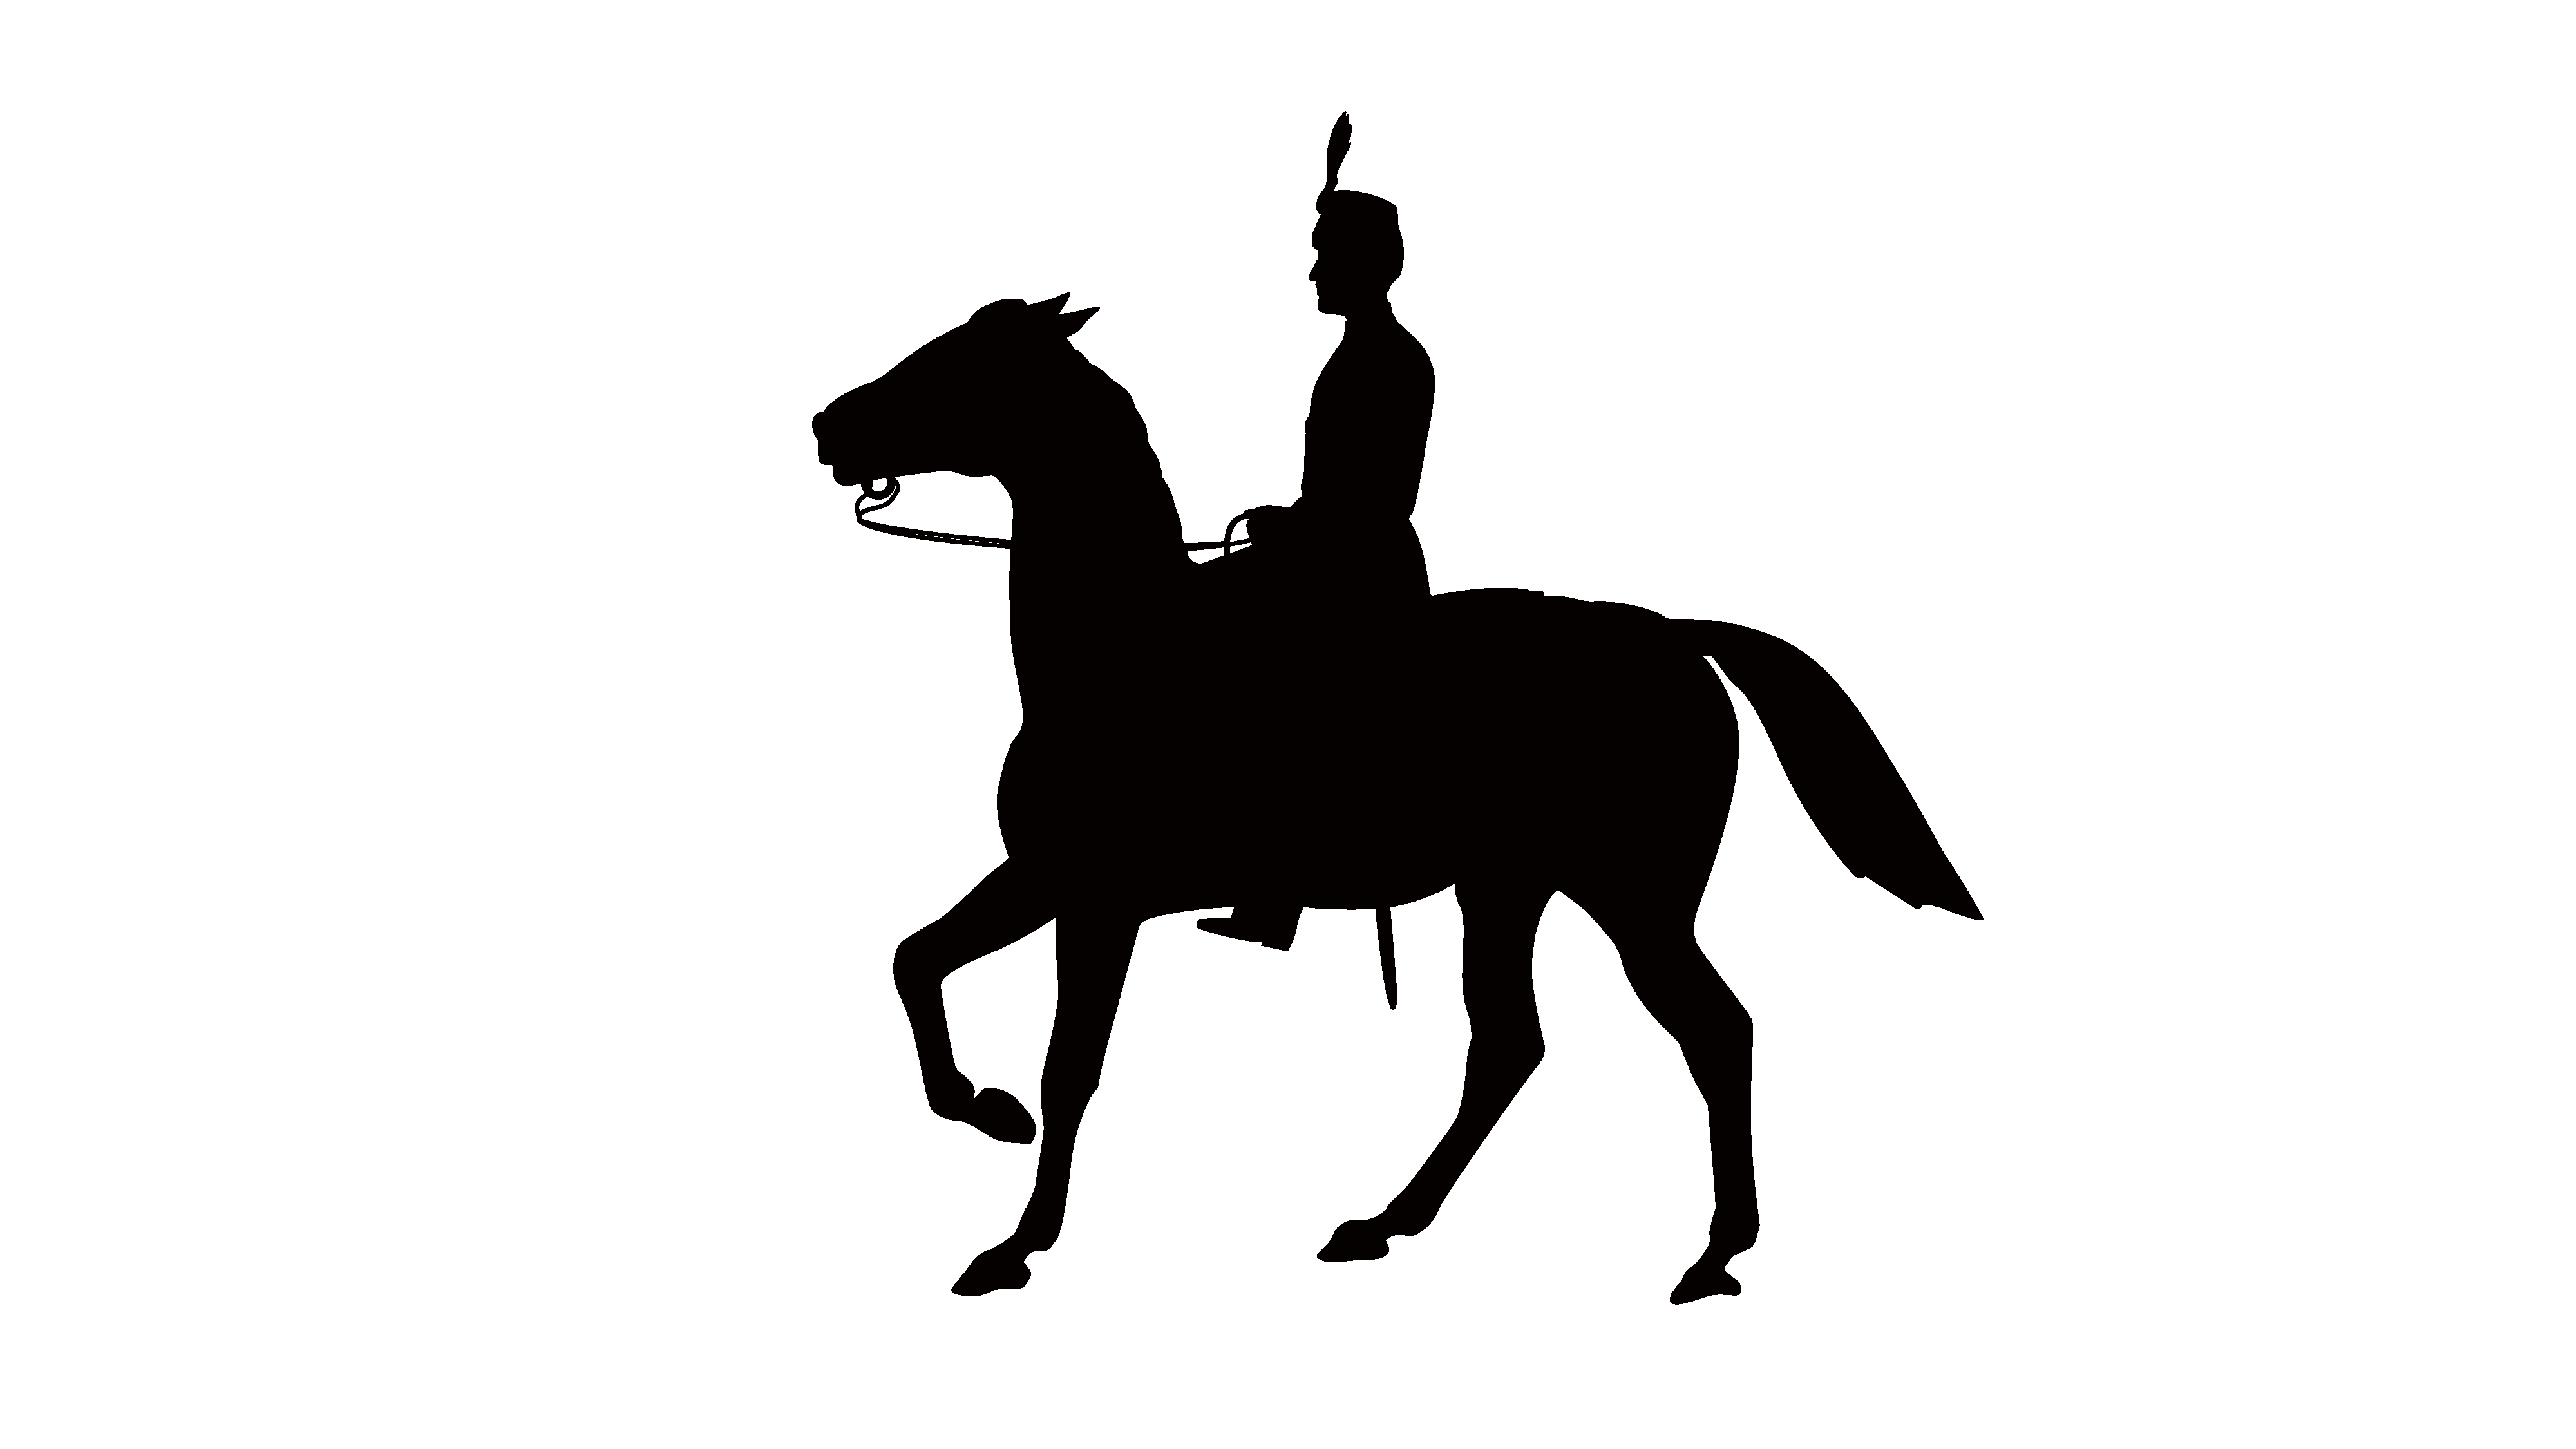
\includegraphics[width=0.6\textwidth]{platforms/horse.pdf}
  \caption*{Horse}
\end{figure}

\begin{figure}[h]
  \centering
  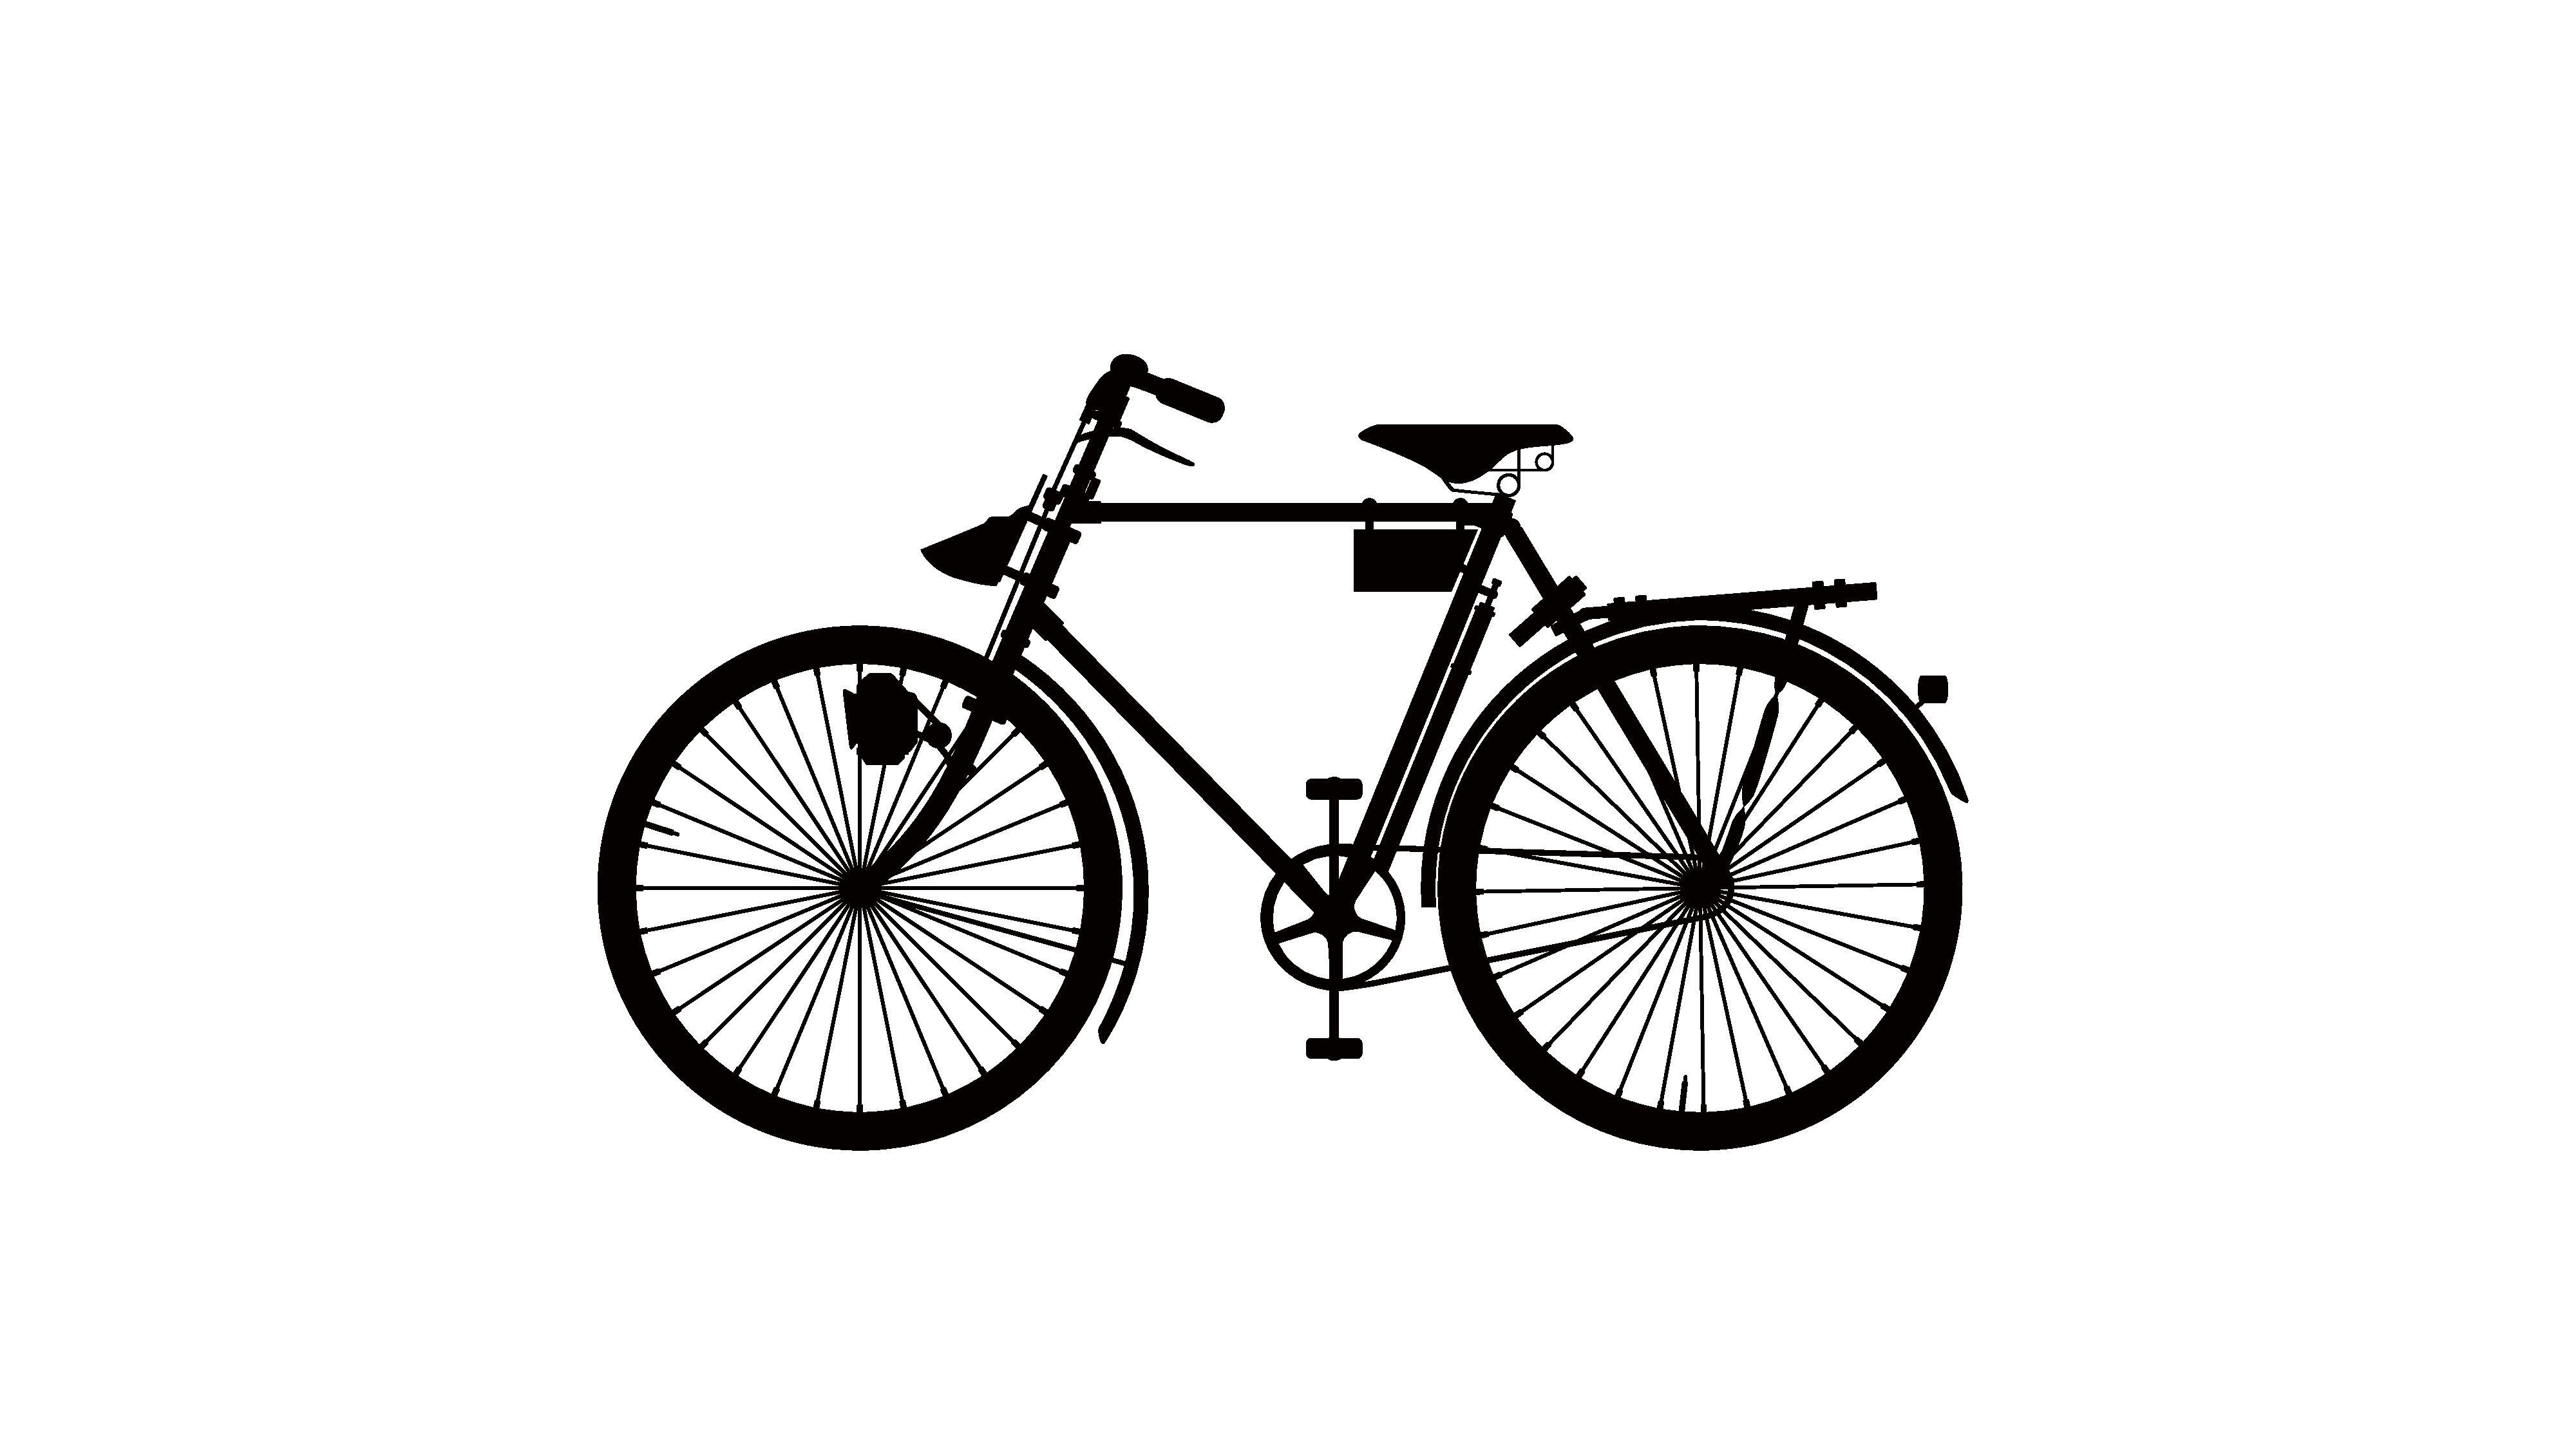
\includegraphics[width=0.5\textwidth]{platforms/bicycle.pdf}
  \caption*{Bicycle}
\end{figure}

\begin{figure}[h]
  \centering
  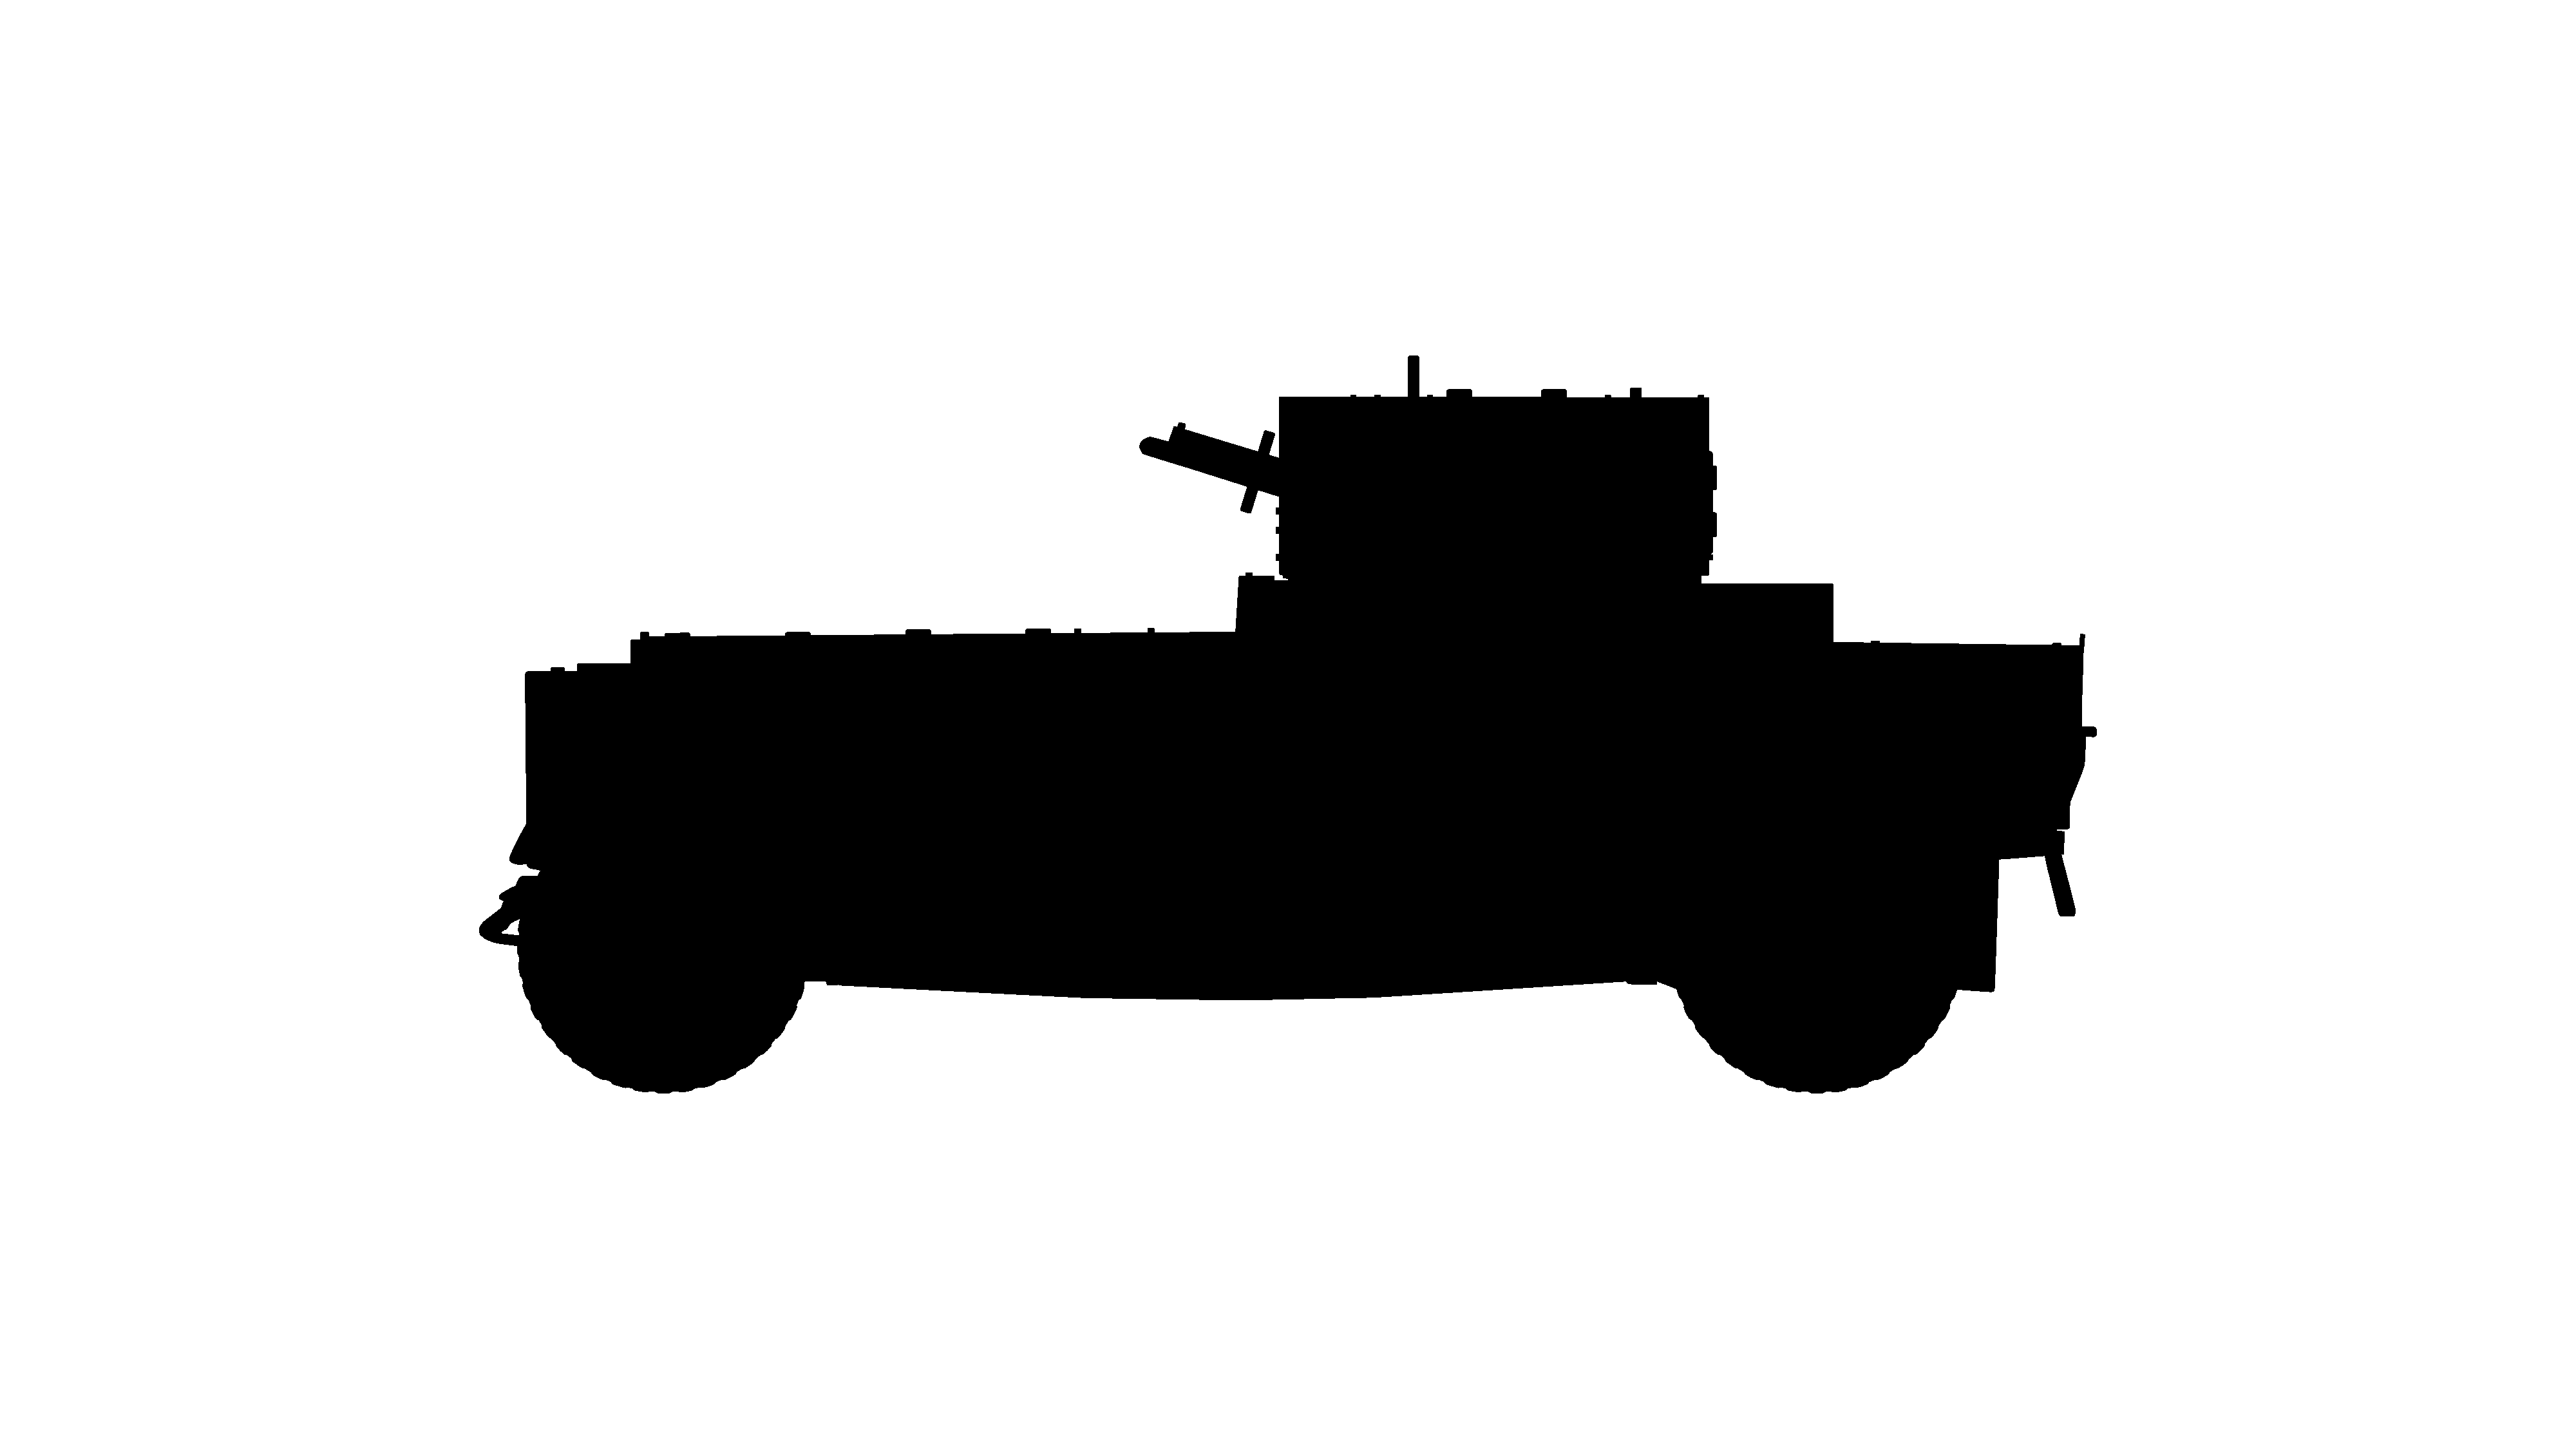
\includegraphics[width=0.7\textwidth]{platforms/rolls-royce.pdf}
  \caption*{Rolls Royce armoured car}
\end{figure}

\begin{figure}[h]
  \centering
  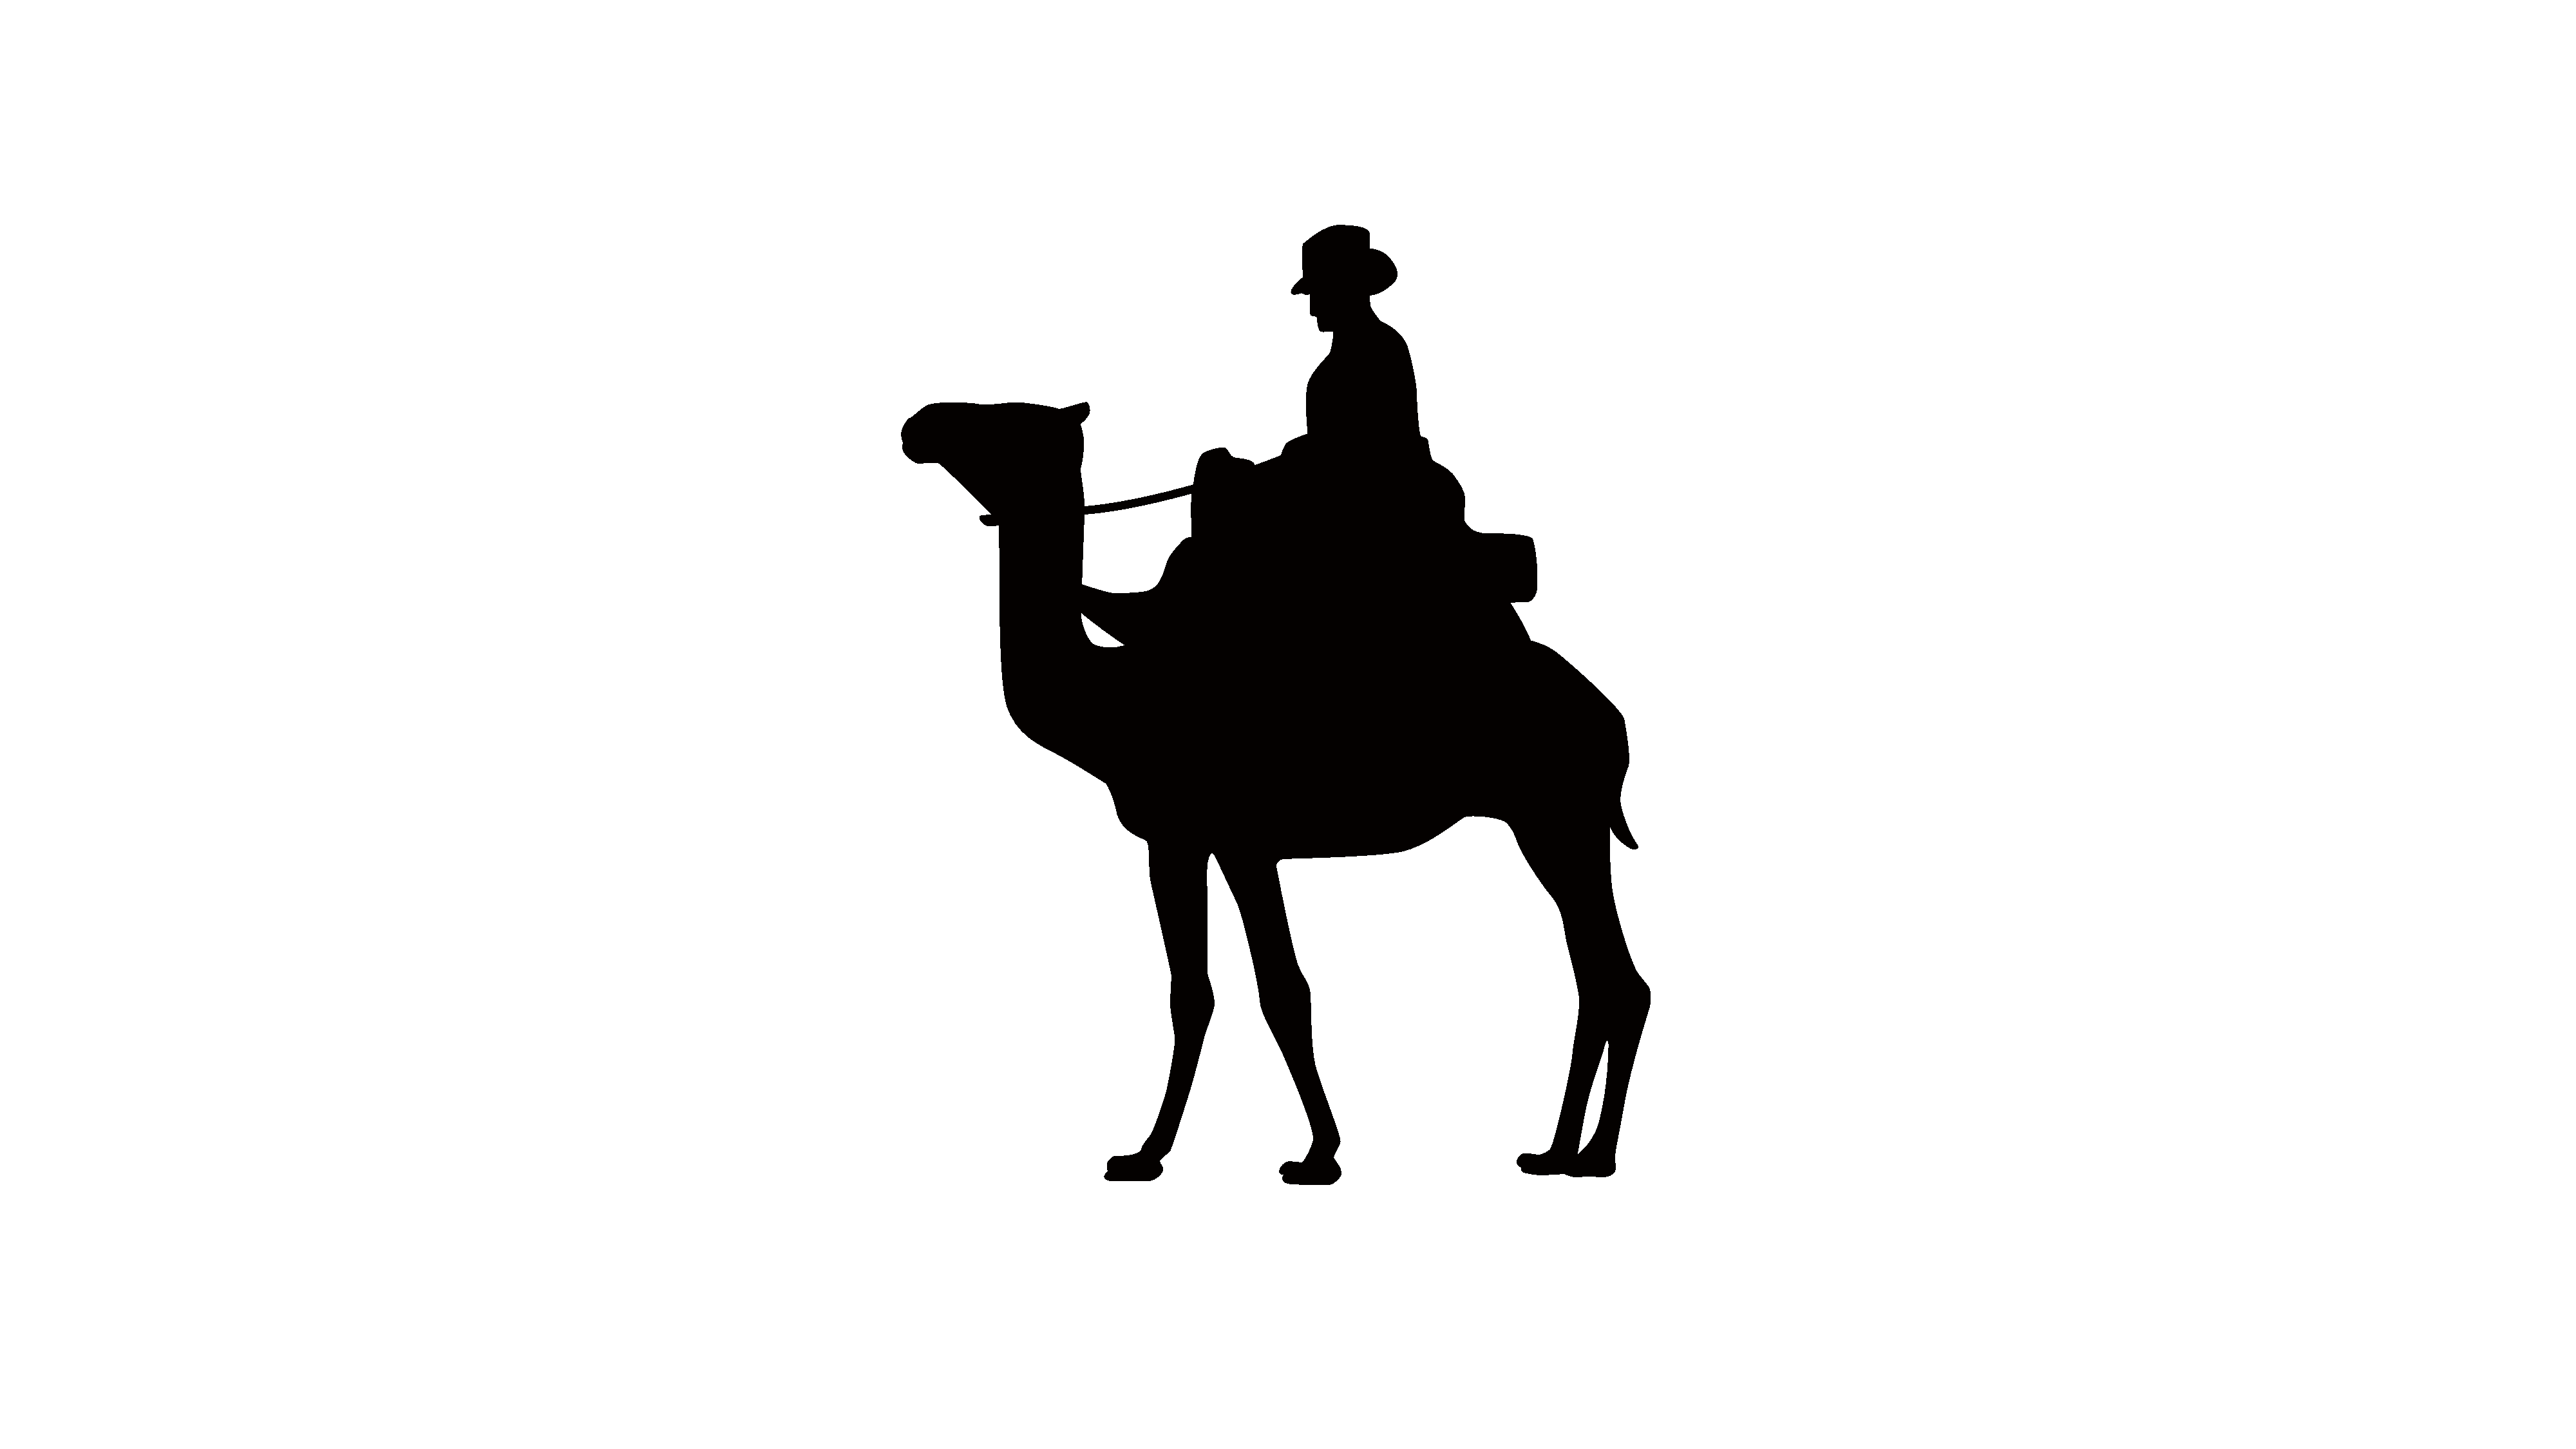
\includegraphics[width=0.5\textwidth]{platforms/camel.pdf}
  \caption*{Camel}
\end{figure}

\begin{figure}[h]
  \centering
  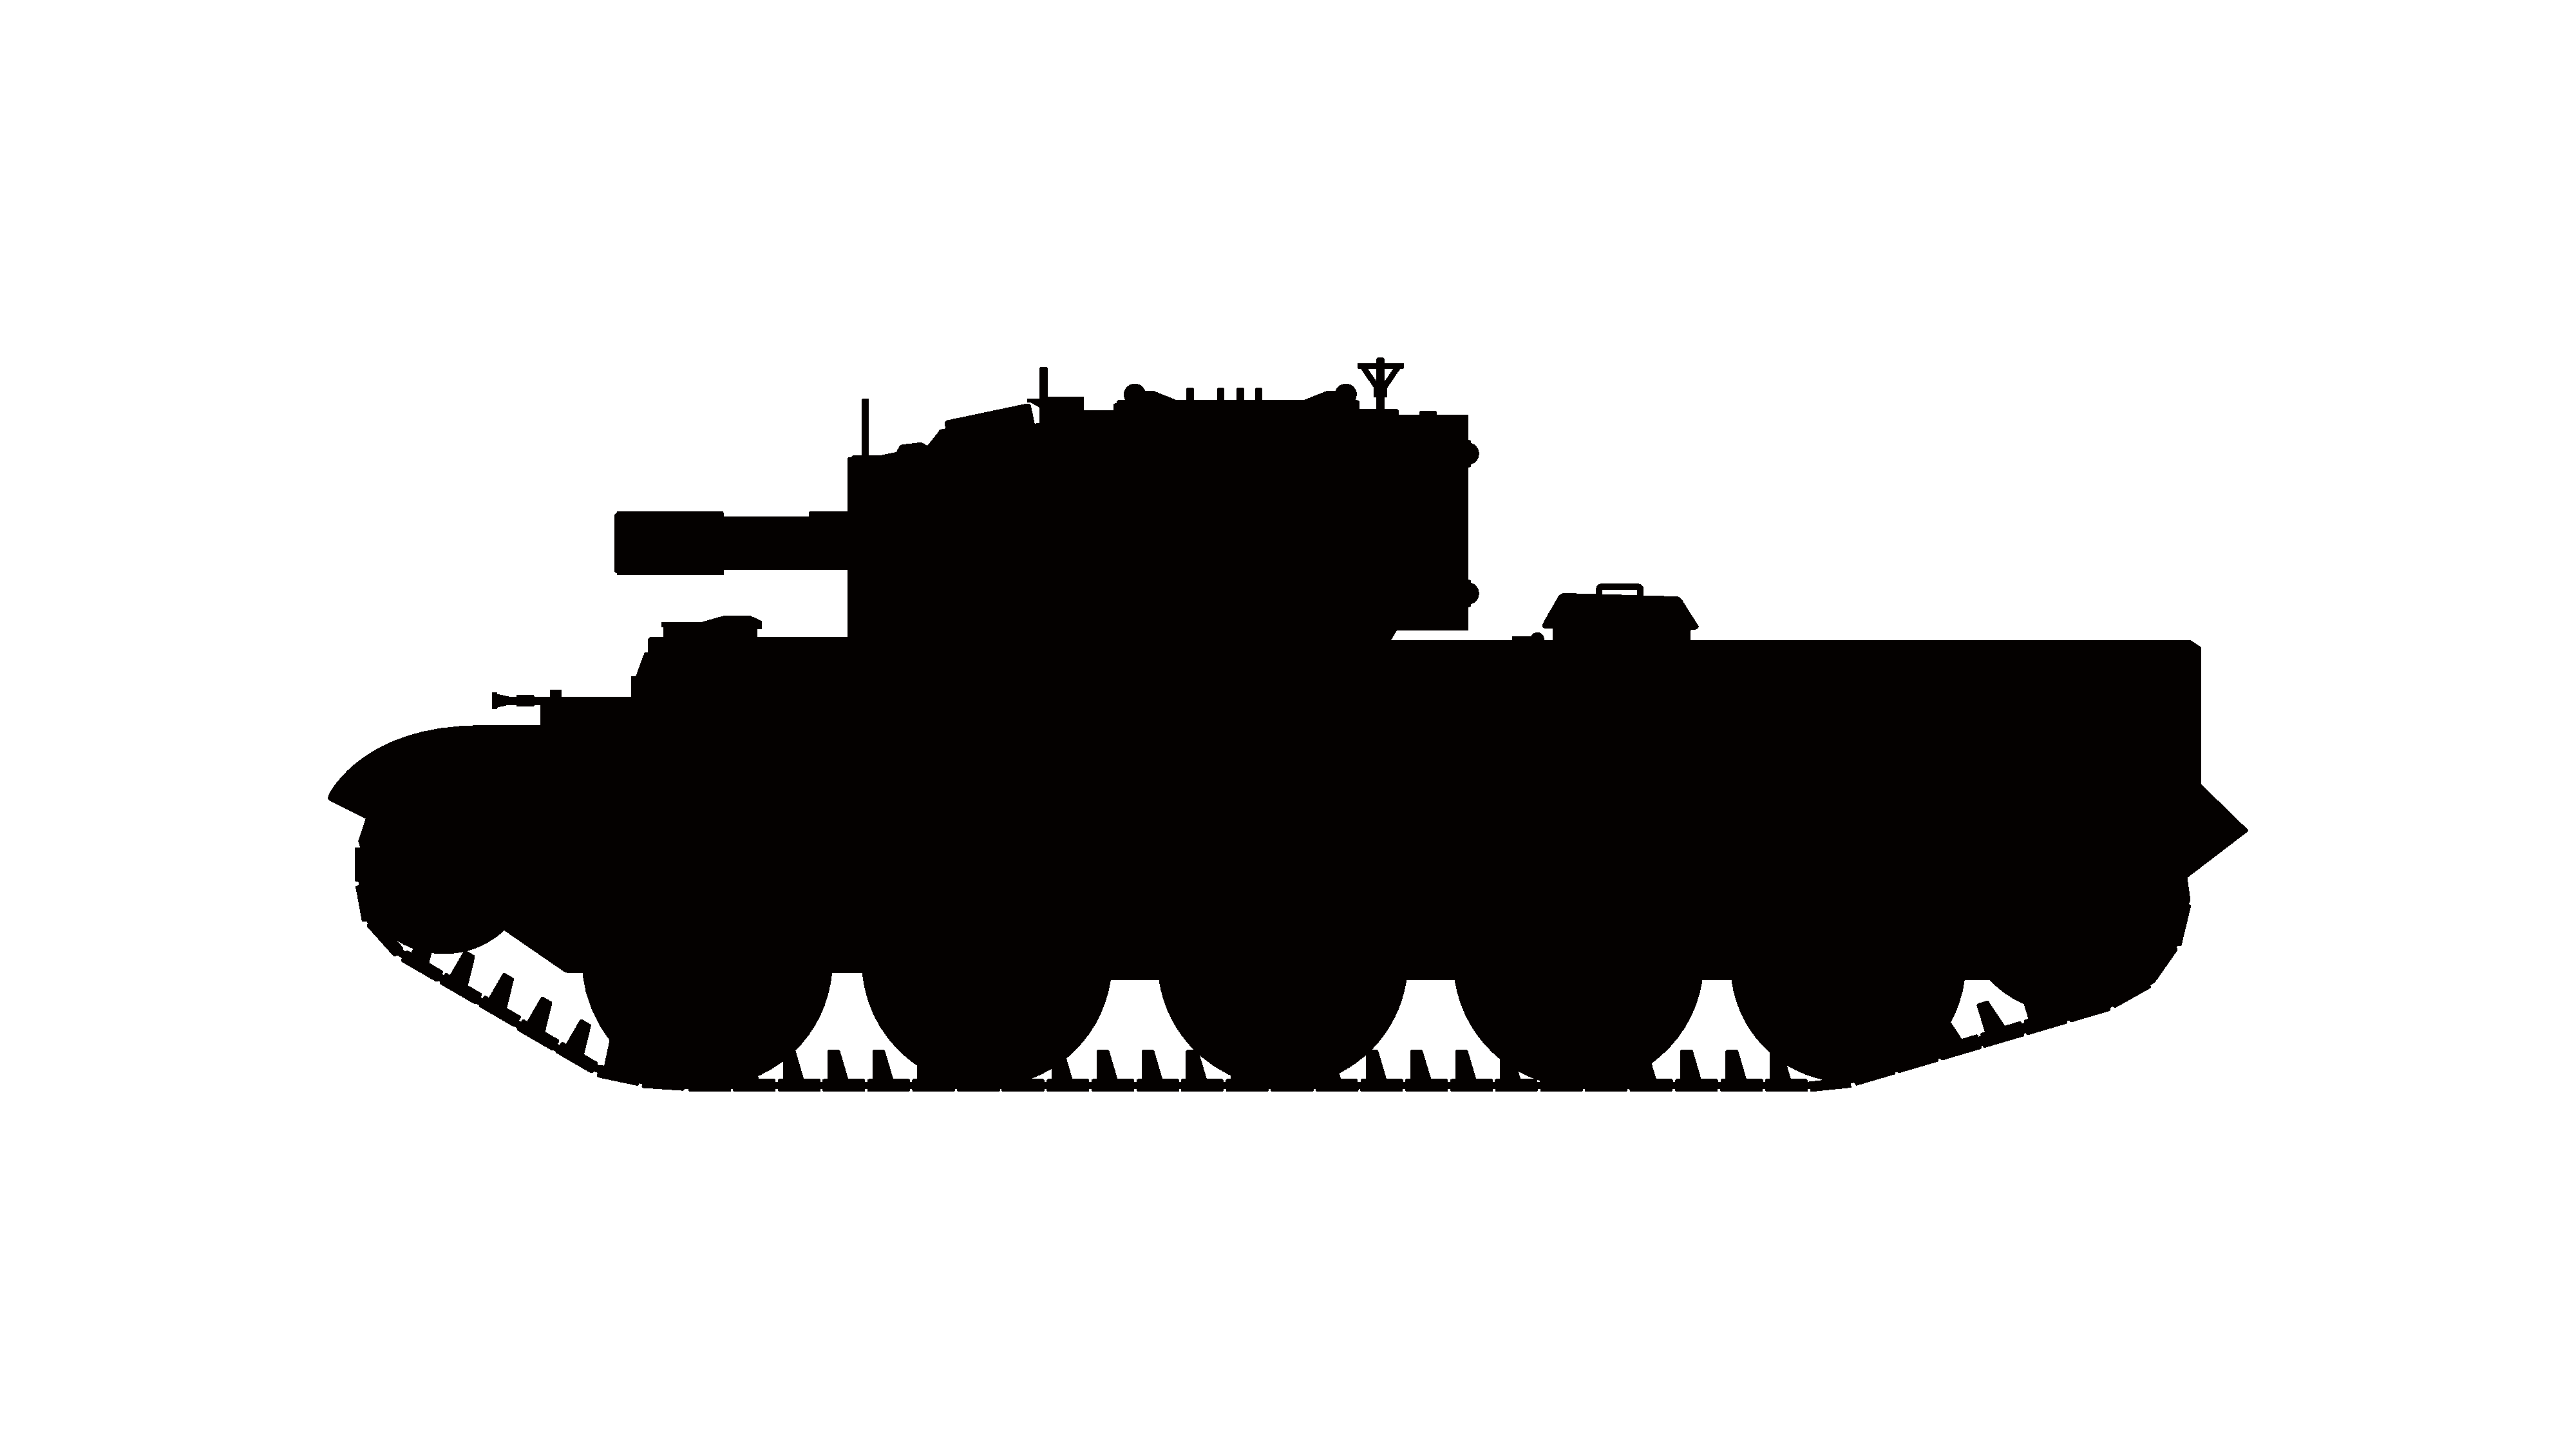
\includegraphics[width=0.7\textwidth]{platforms/cromwell.pdf}
  \caption*{Cromwell}
\end{figure}

\begin{figure}[h]
  \centering
  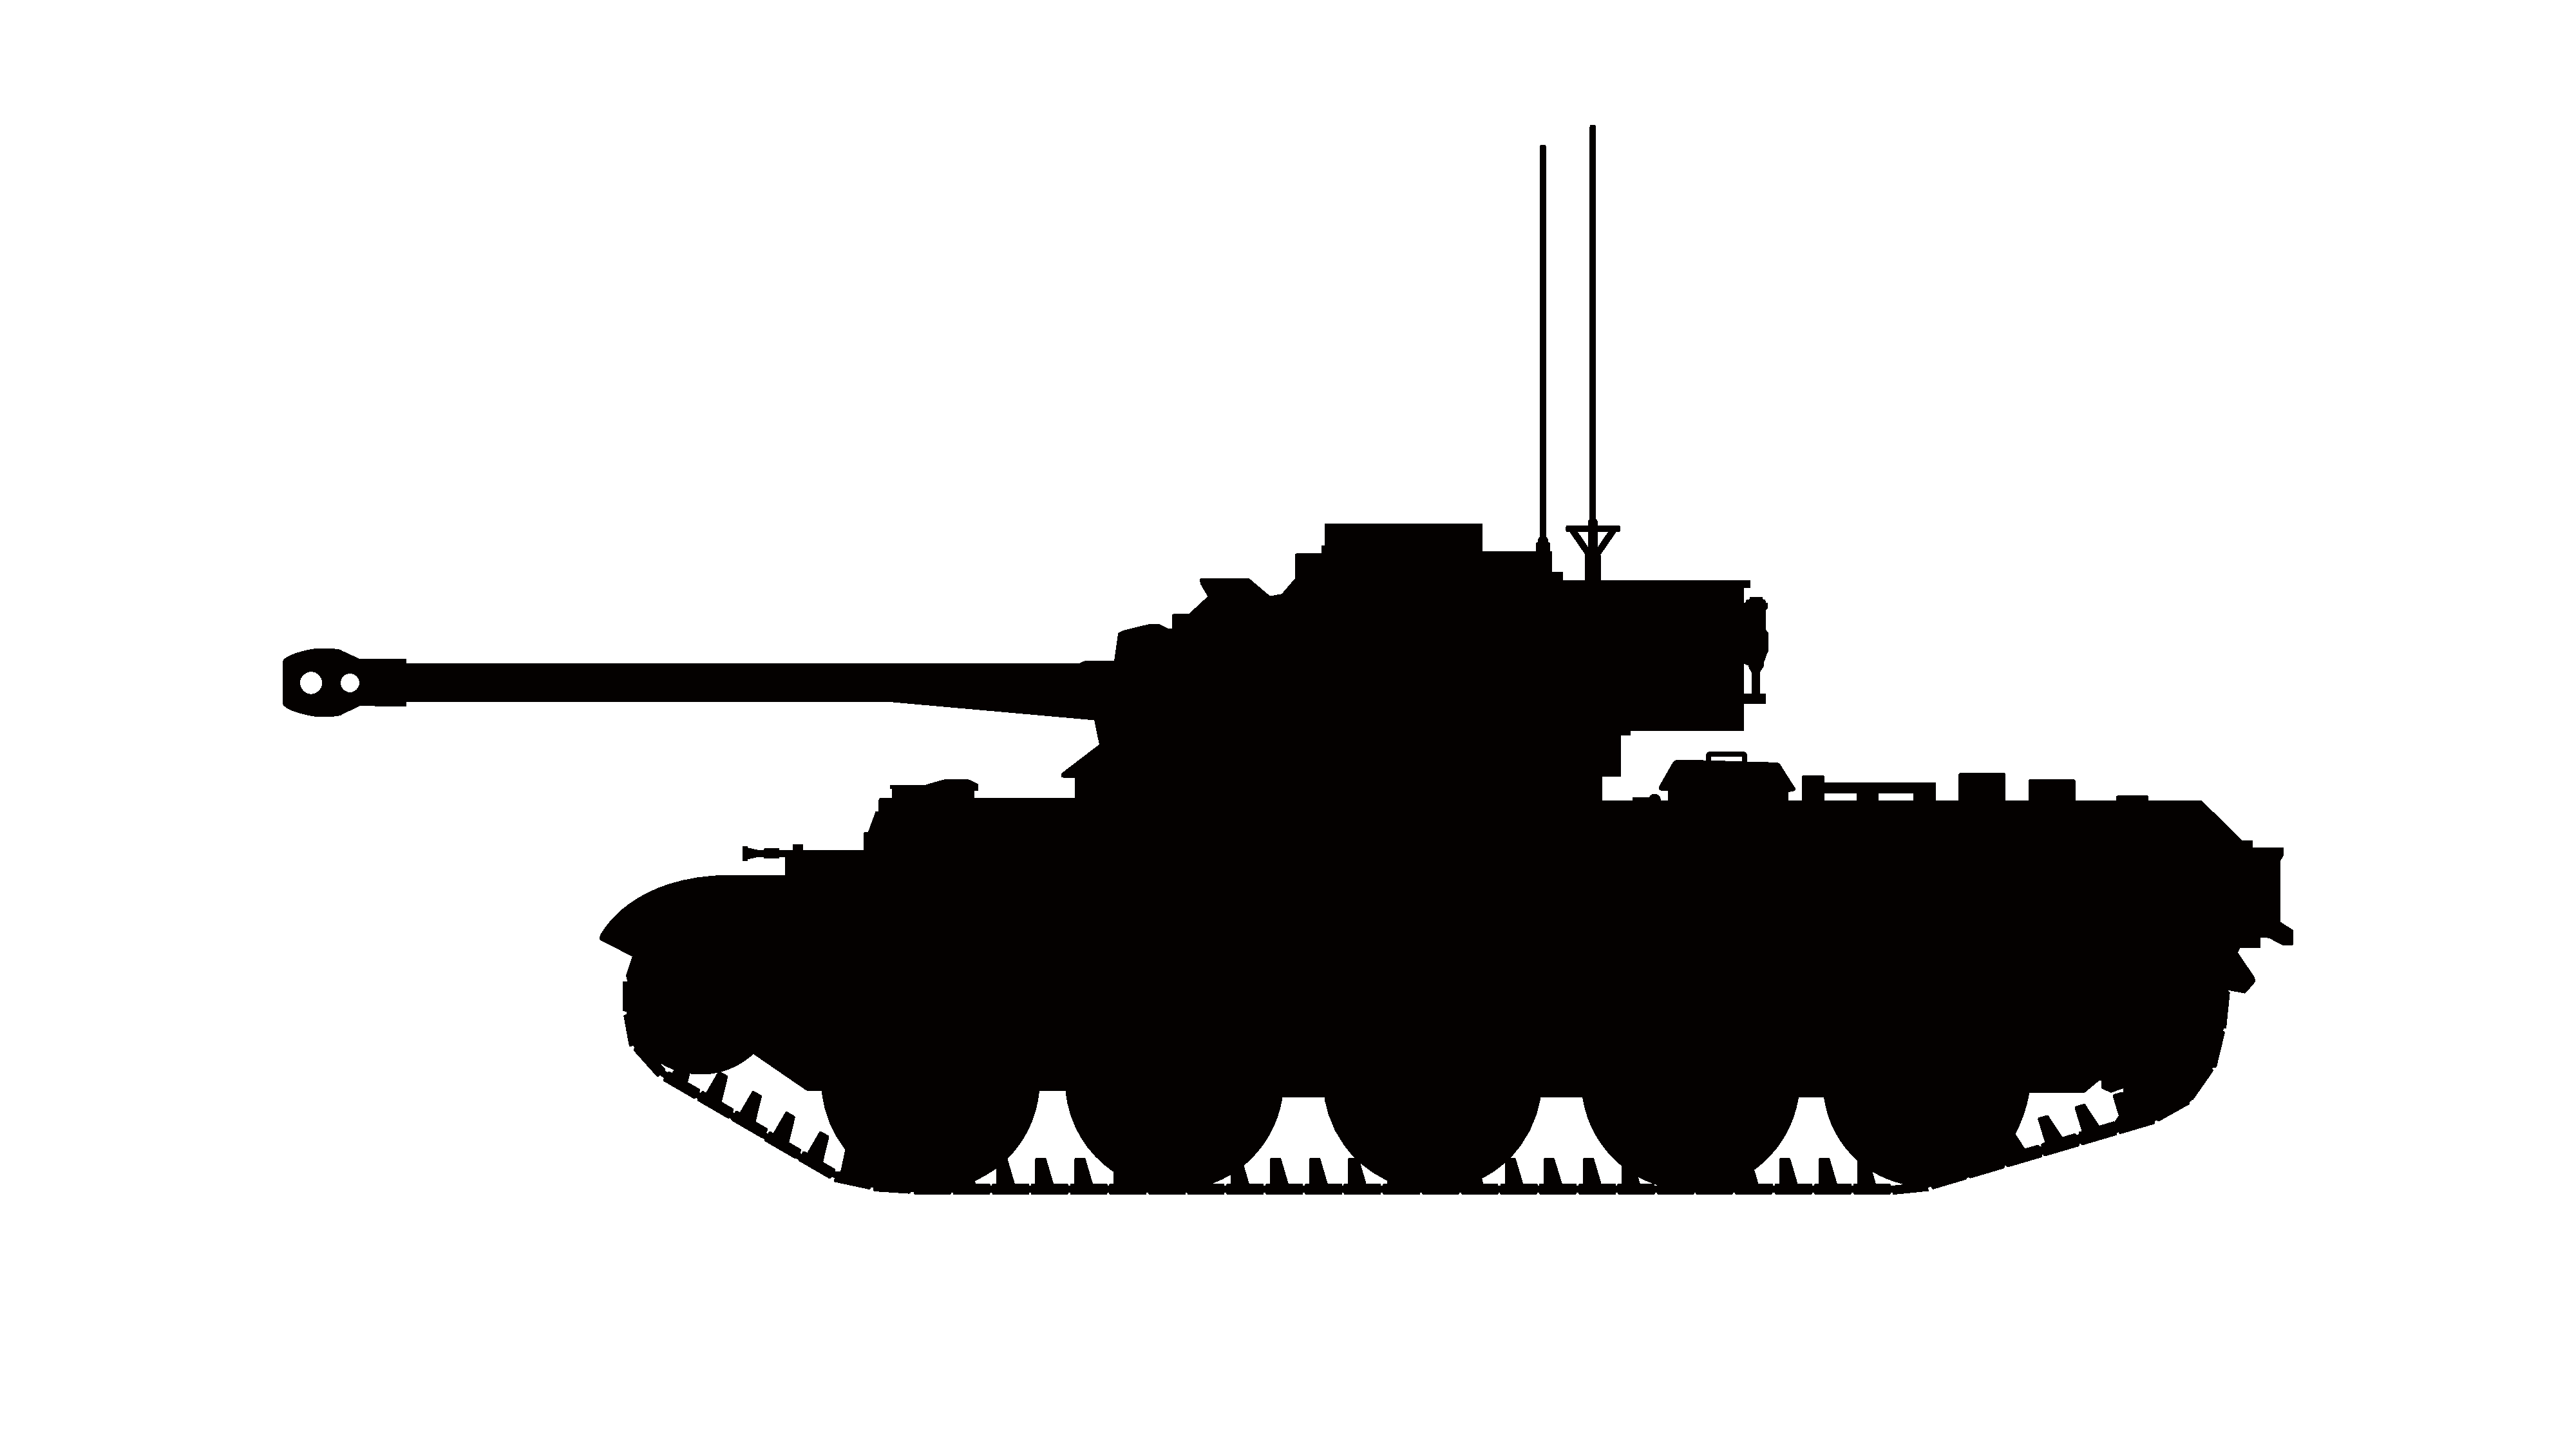
\includegraphics[width=0.7\textwidth]{platforms/comet.pdf}
  \caption*{Comet}
\end{figure}

\begin{figure}[h]
  \centering
  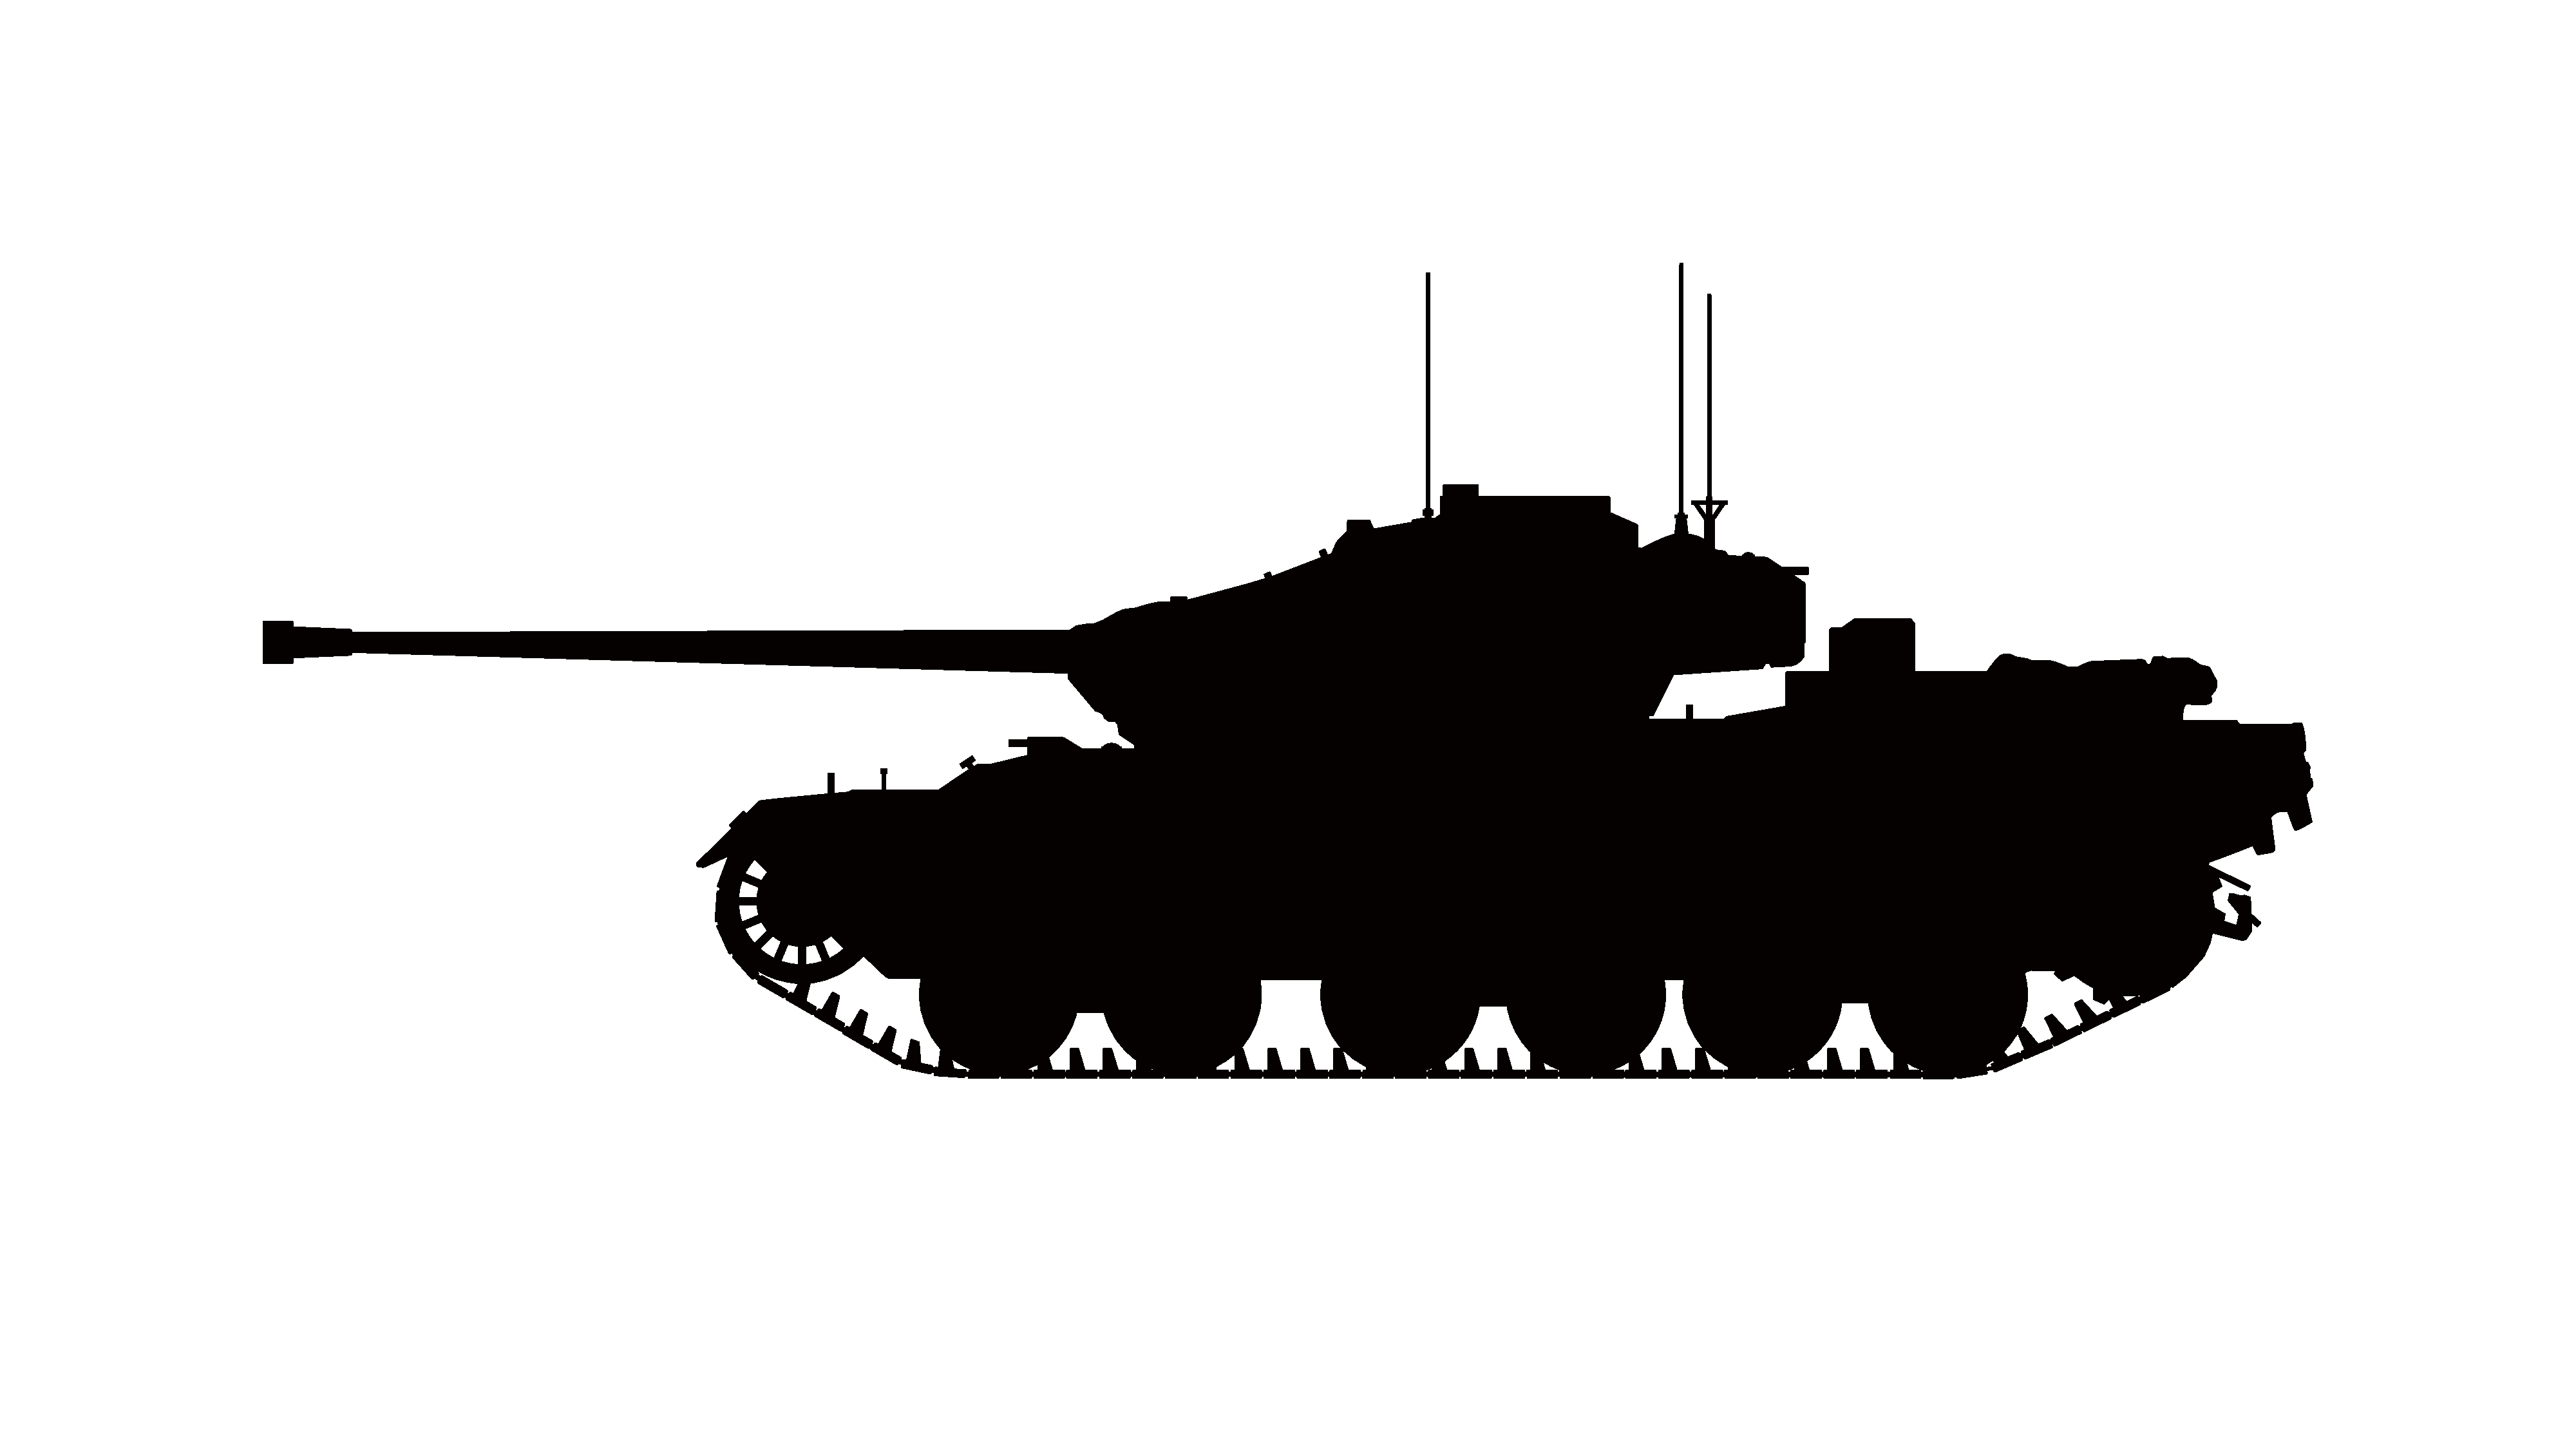
\includegraphics[width=0.7\textwidth]{platforms/centurion.pdf}
  \caption*{Centurion}
\end{figure}

\begin{figure}[h]
  \centering
  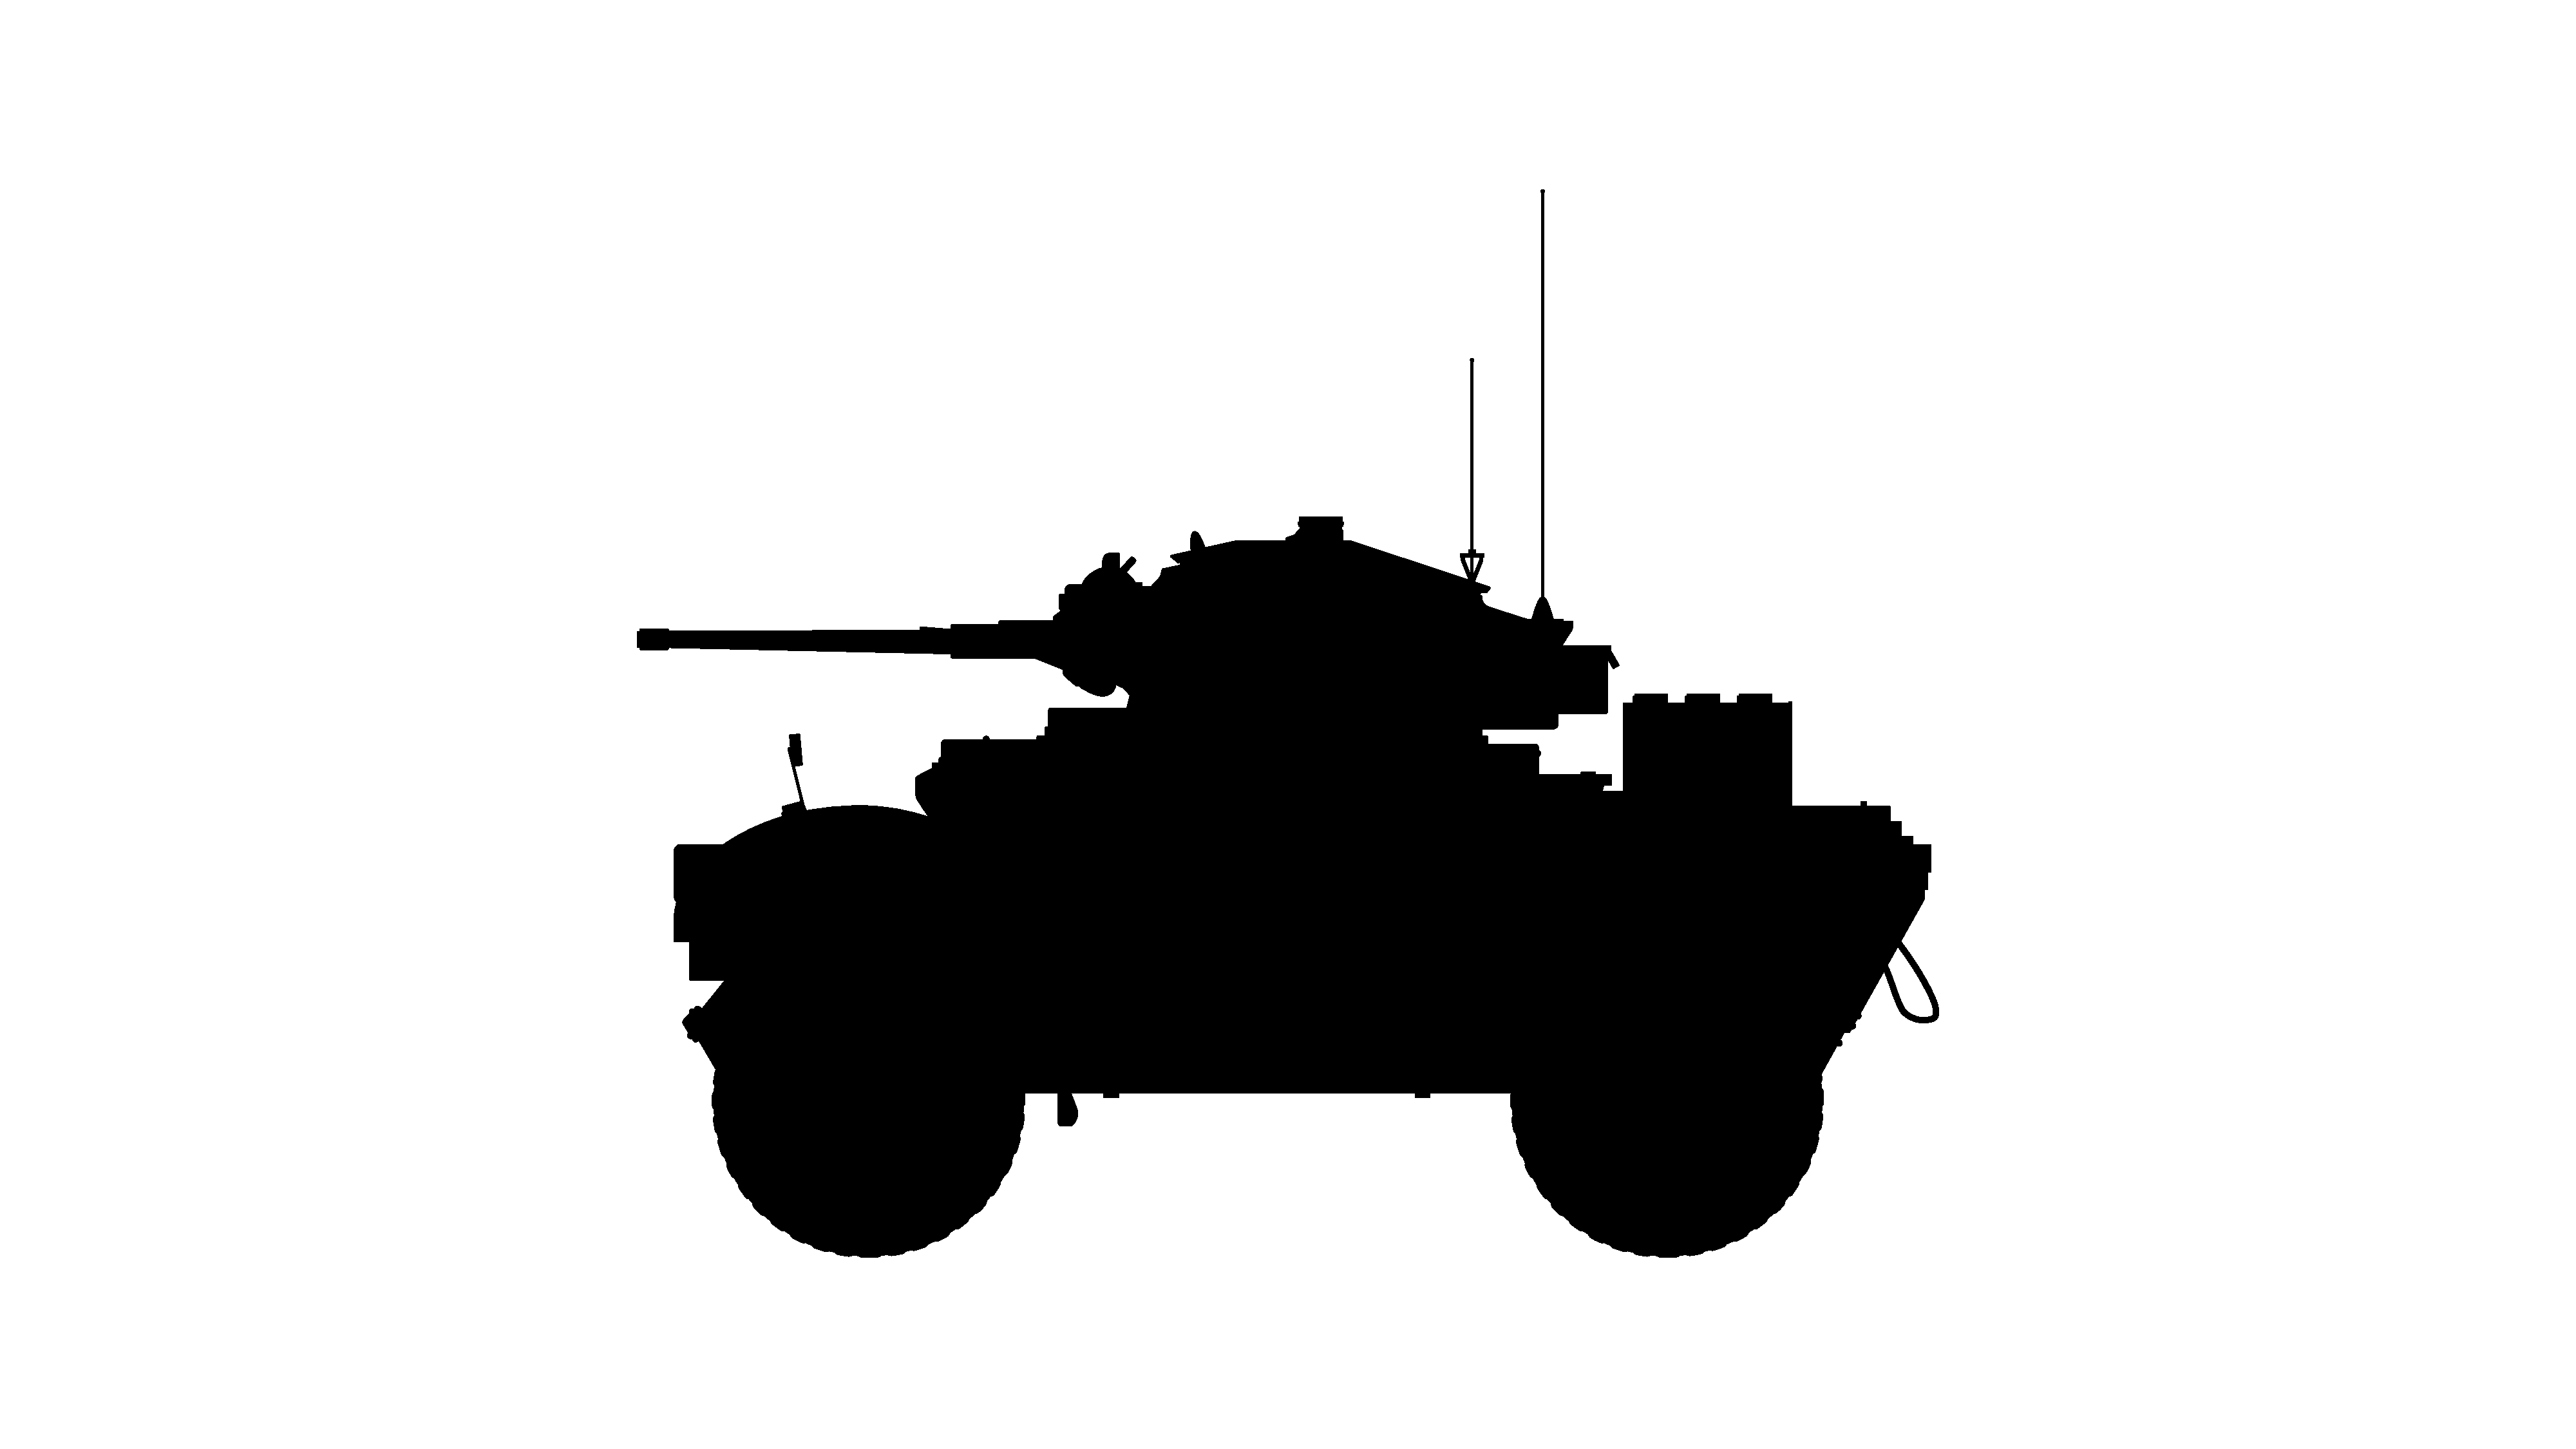
\includegraphics[width=0.7\textwidth]{platforms/daimler-armoured-car.pdf}
  \caption*{Daimler armoured car}
\end{figure}

\begin{figure}[h]
  \centering
  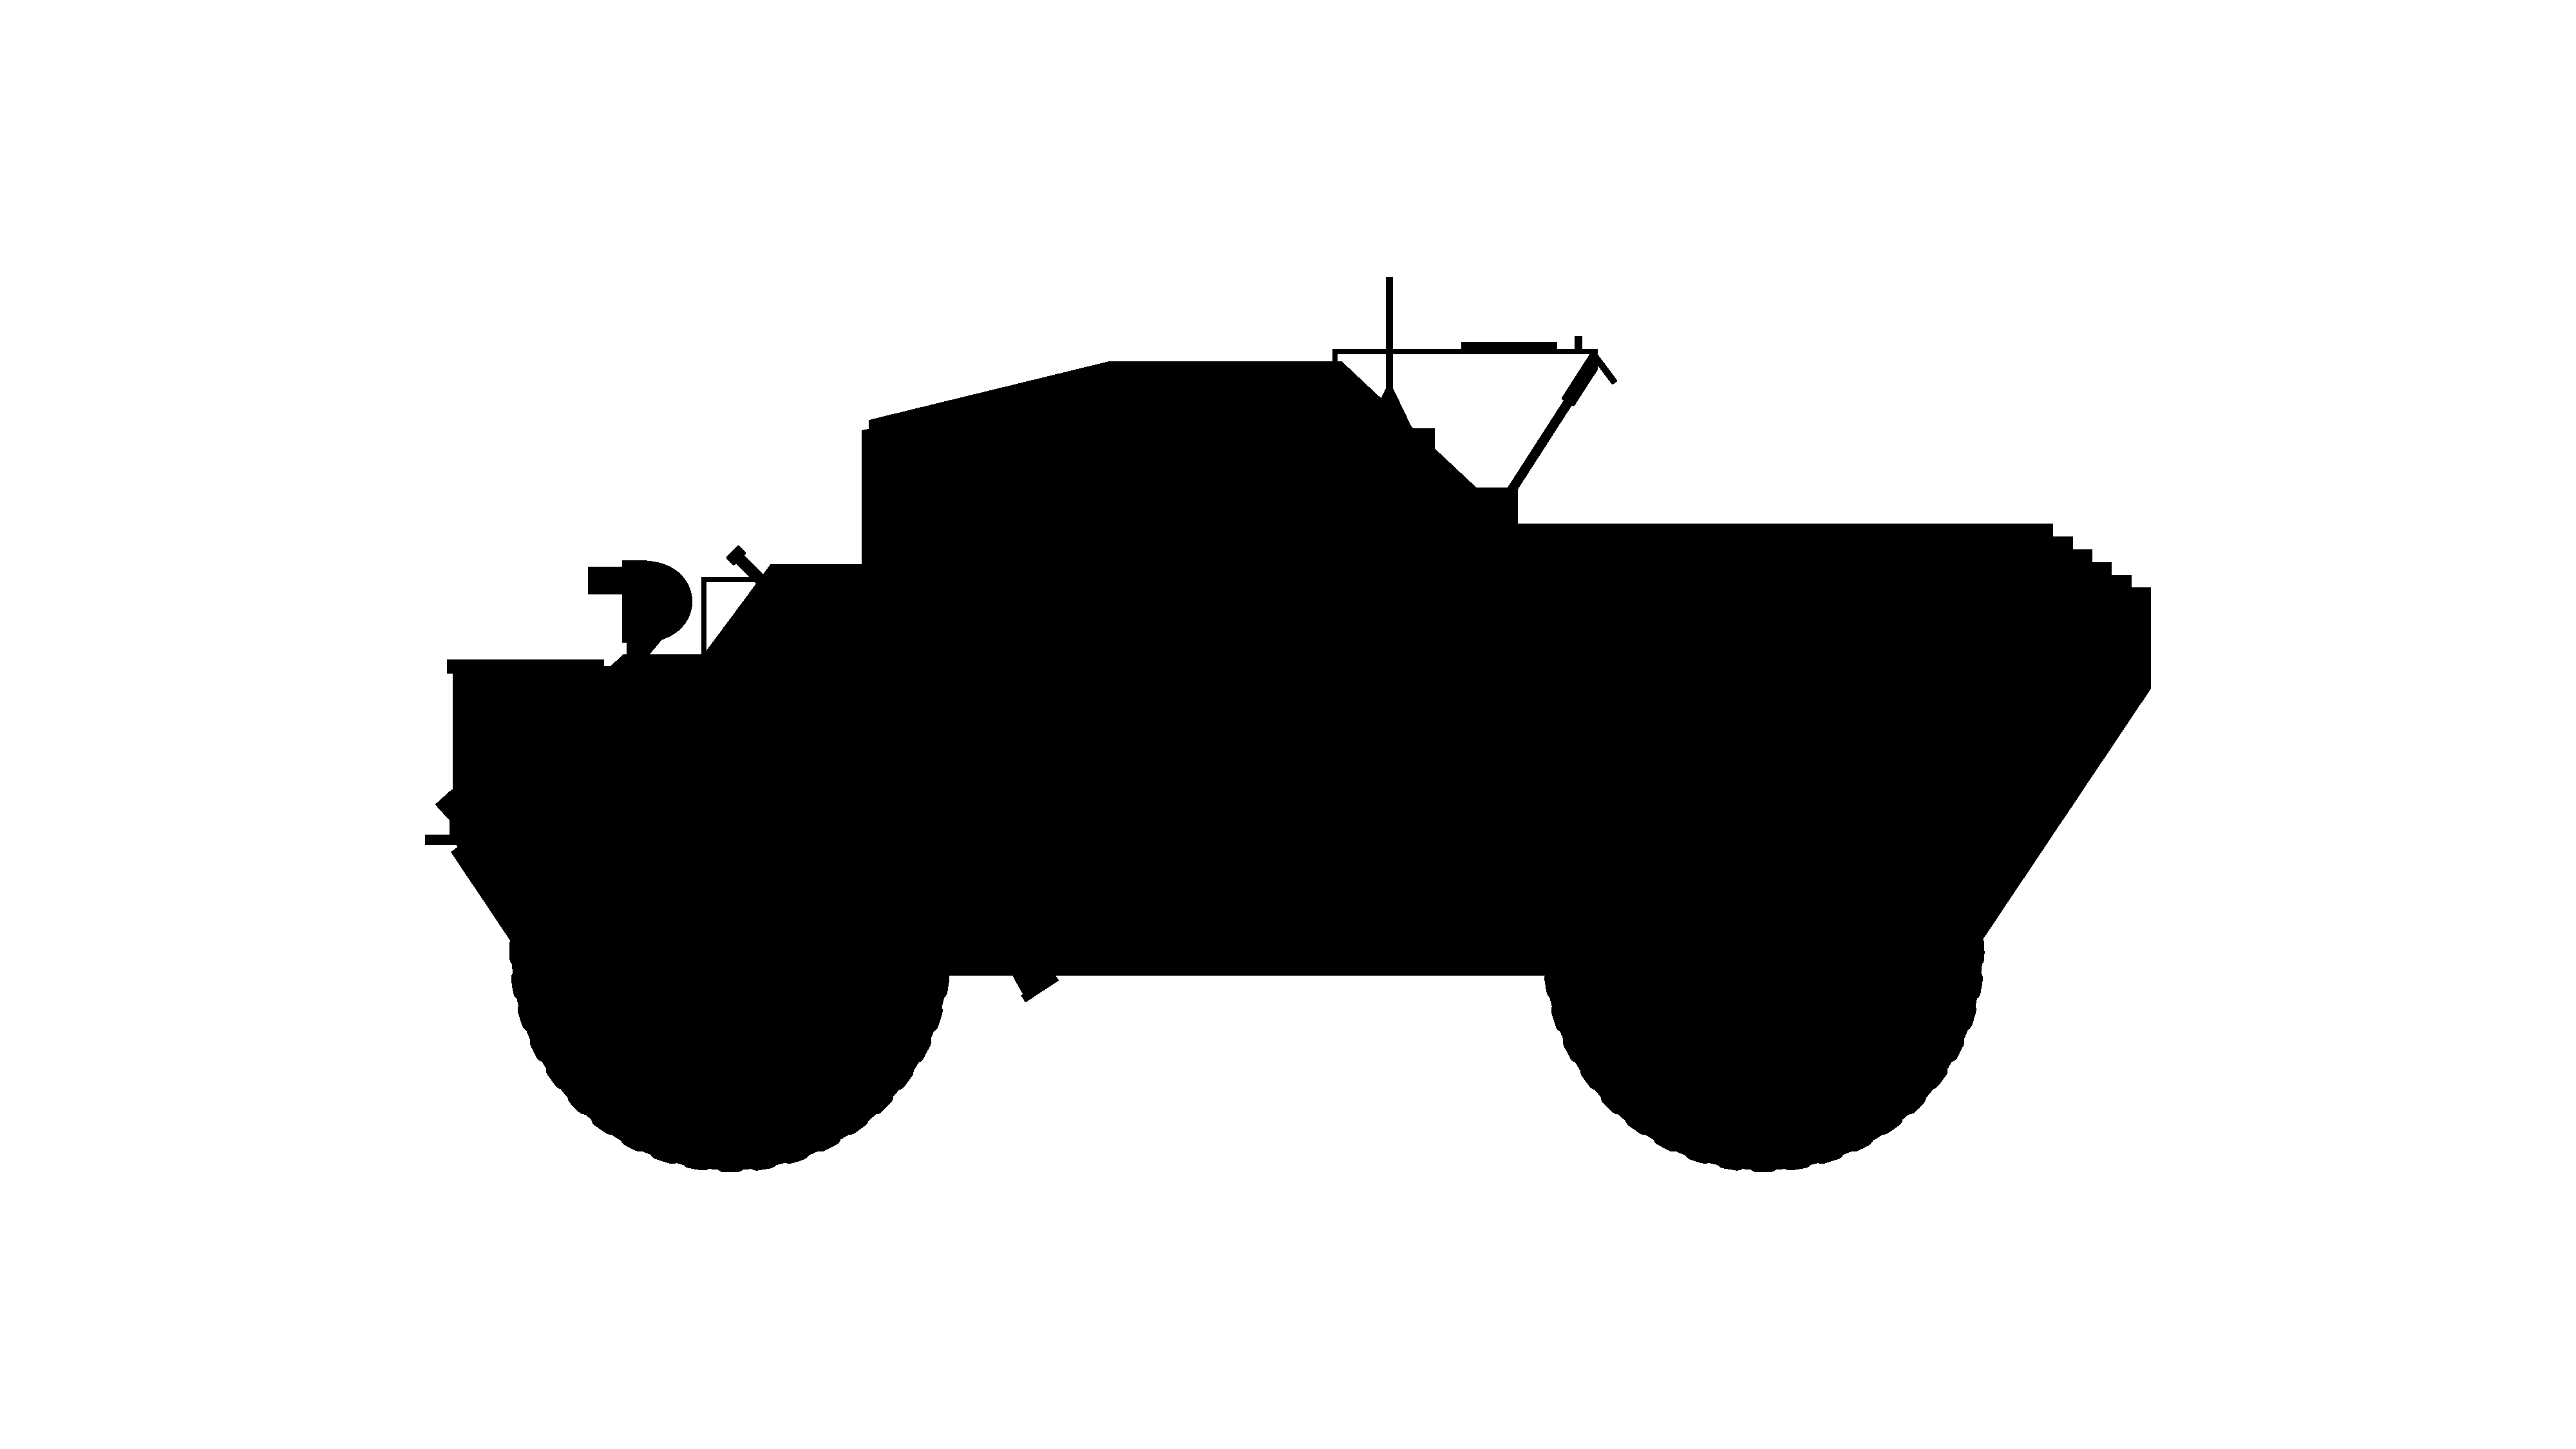
\includegraphics[width=0.7\textwidth]{platforms/daimler-scout.pdf}
  \caption*{Daimler scout car}
\end{figure}

\begin{figure}[h]
  \centering
  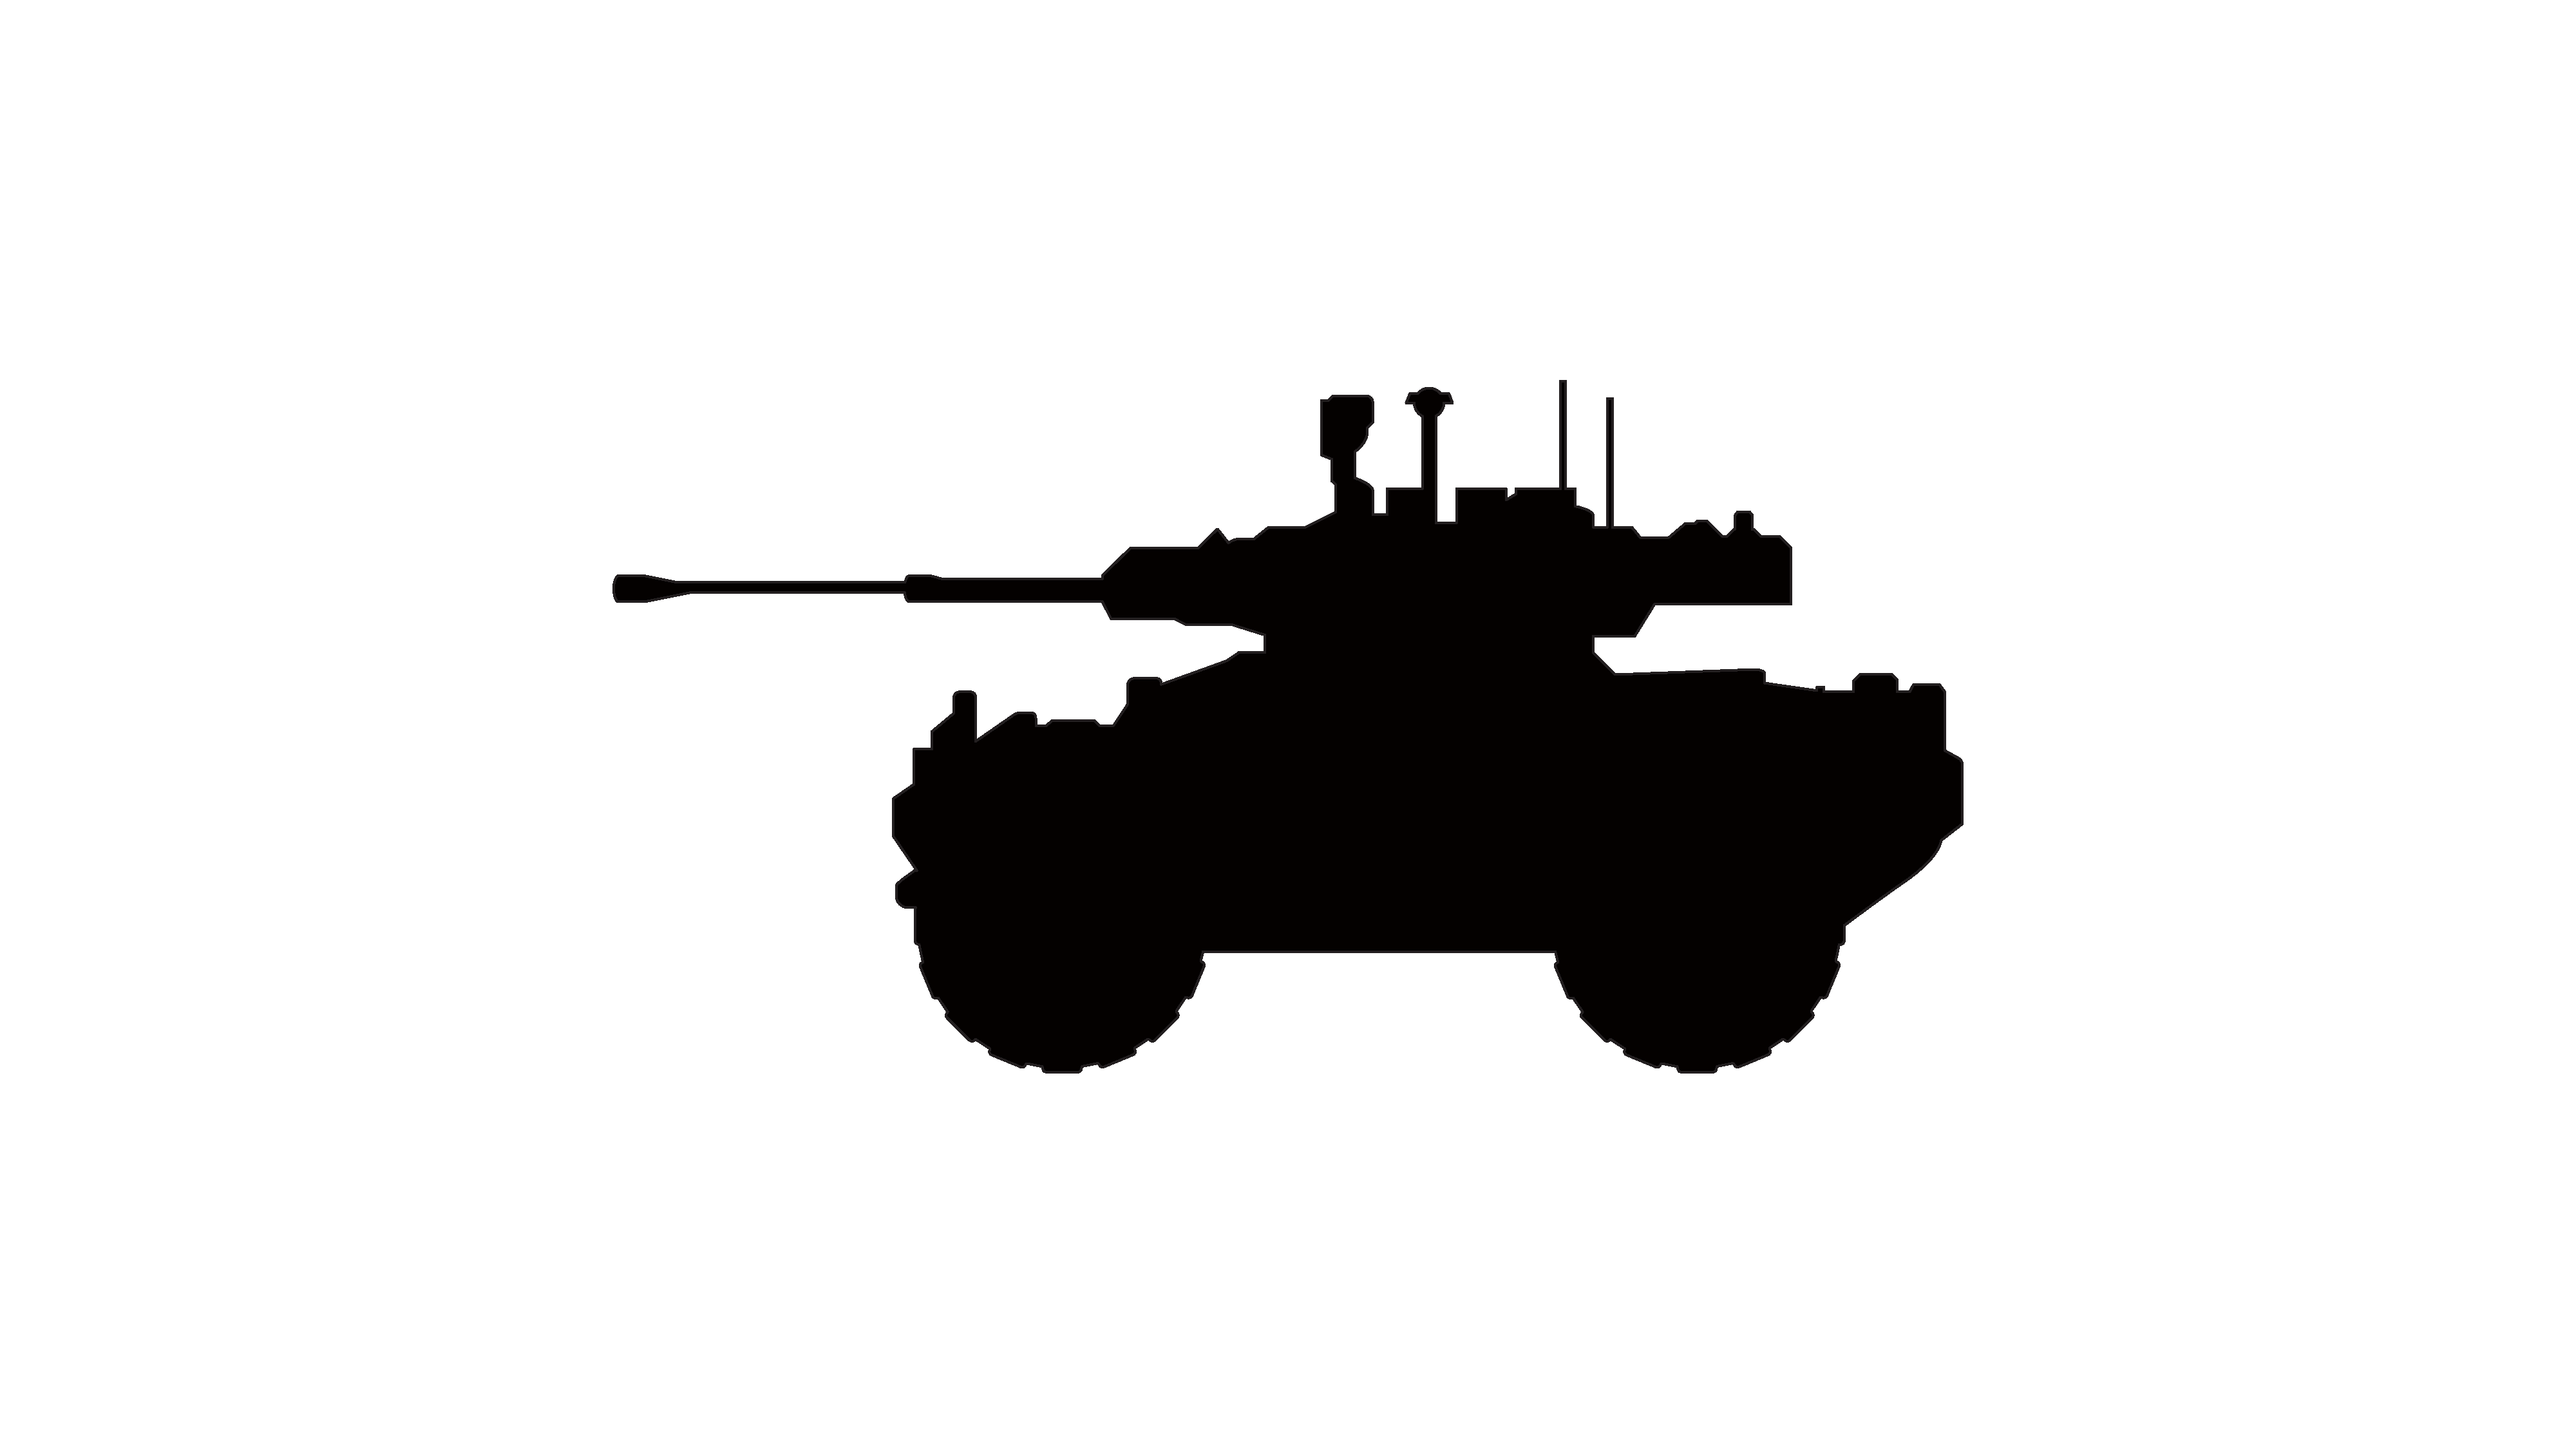
\includegraphics[width=0.7\textwidth]{platforms/fox.pdf}
  \caption*{Fox}
\end{figure}

\begin{figure}[h]
  \centering
  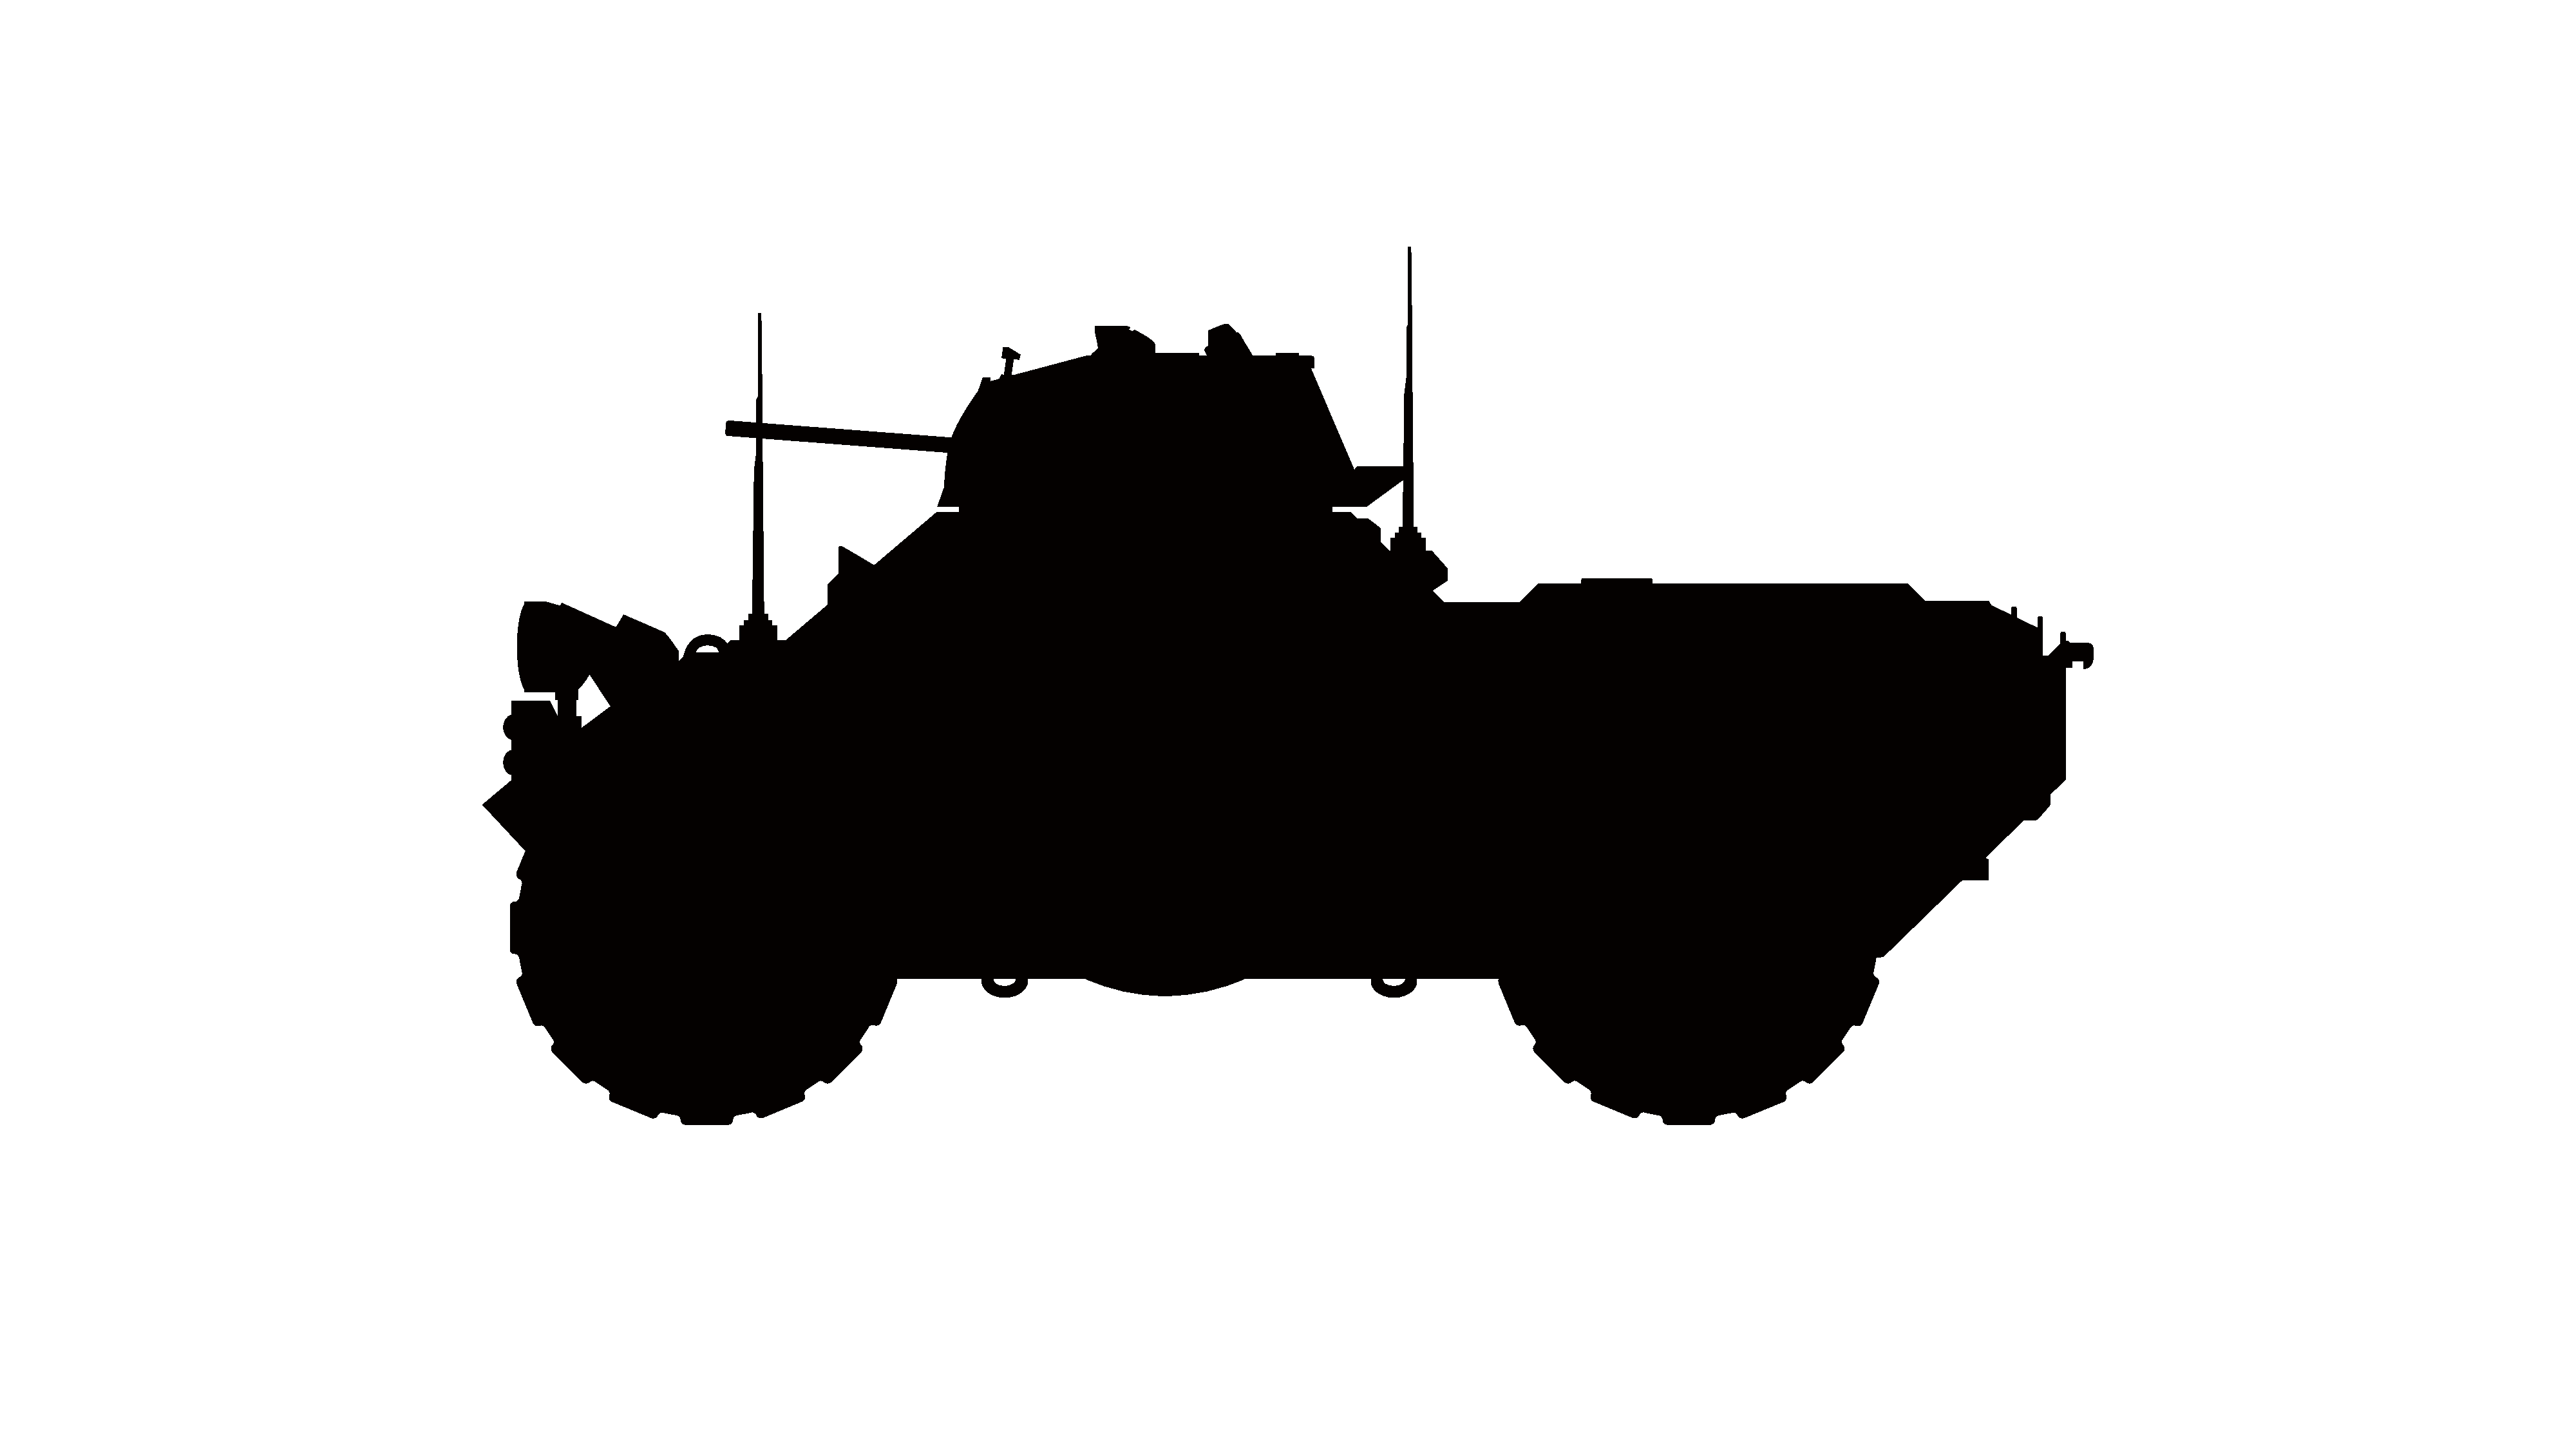
\includegraphics[width=0.7\textwidth]{platforms/ferret.pdf}
  \caption*{Ferret}
\end{figure}

\begin{figure}[h]
  \centering
  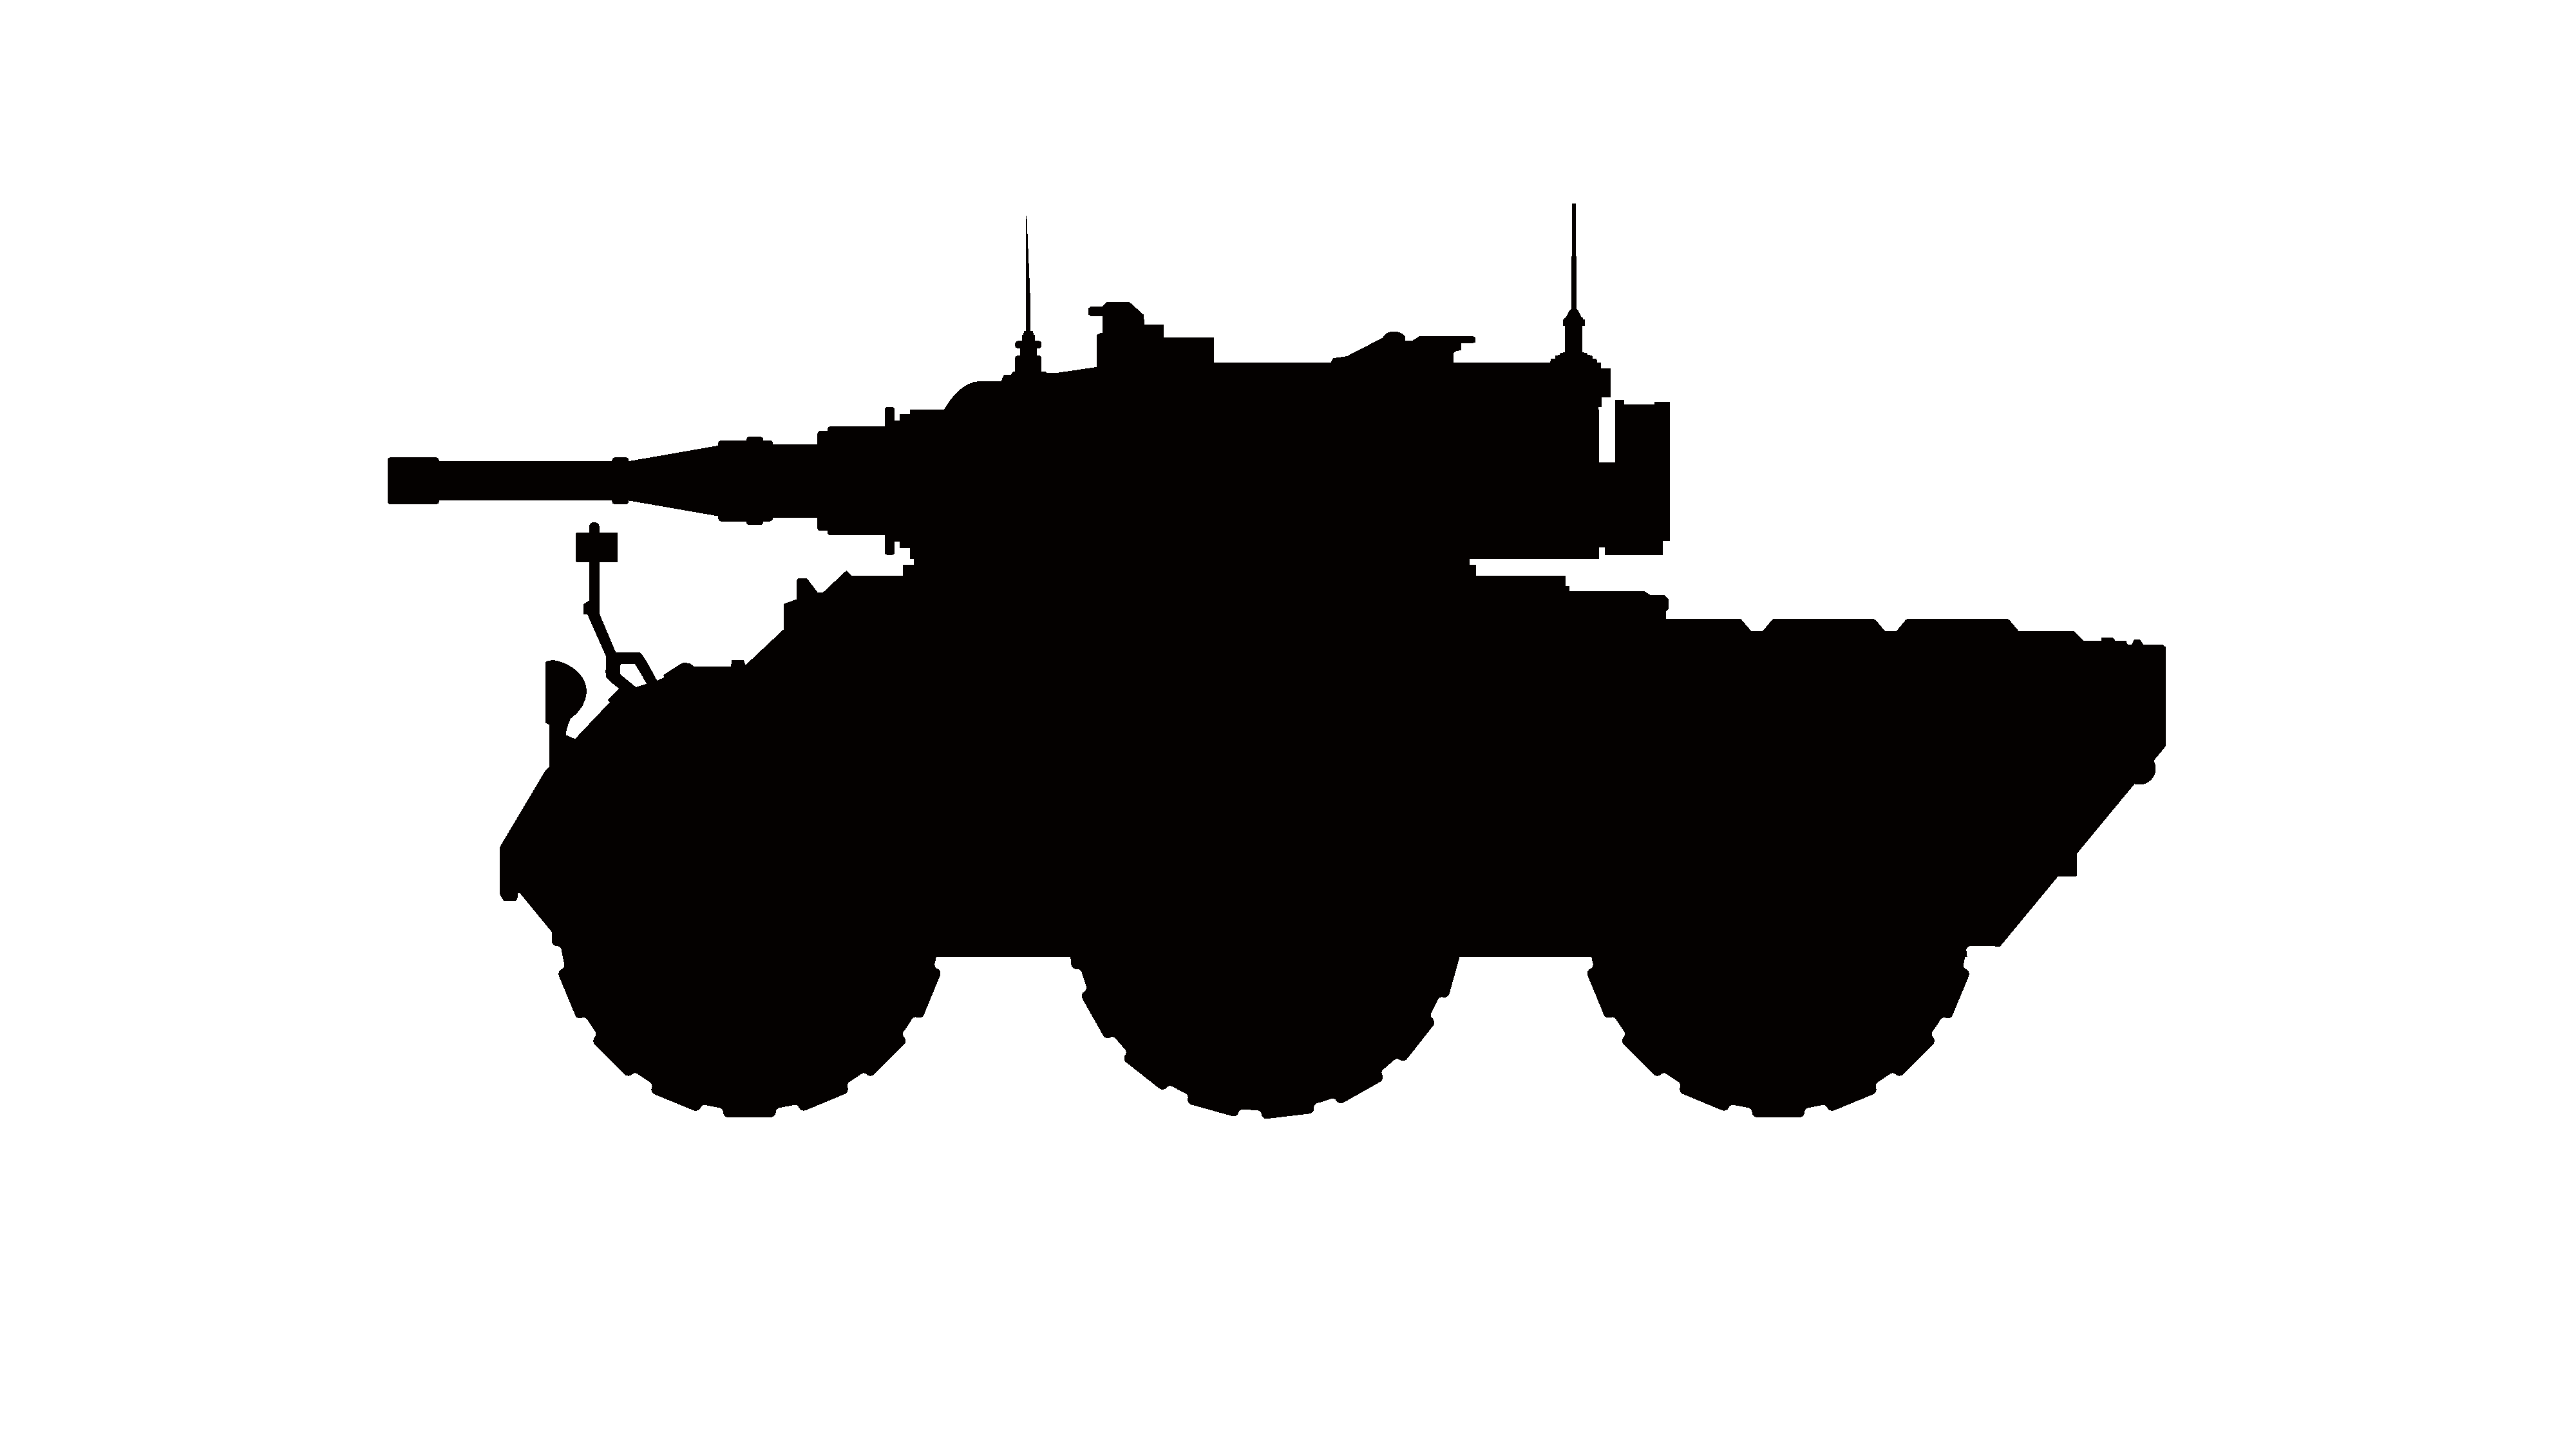
\includegraphics[width=0.7\textwidth]{platforms/saladin.pdf}
  \caption*{Saladin}
\end{figure}

\begin{figure}[h]
  \centering
  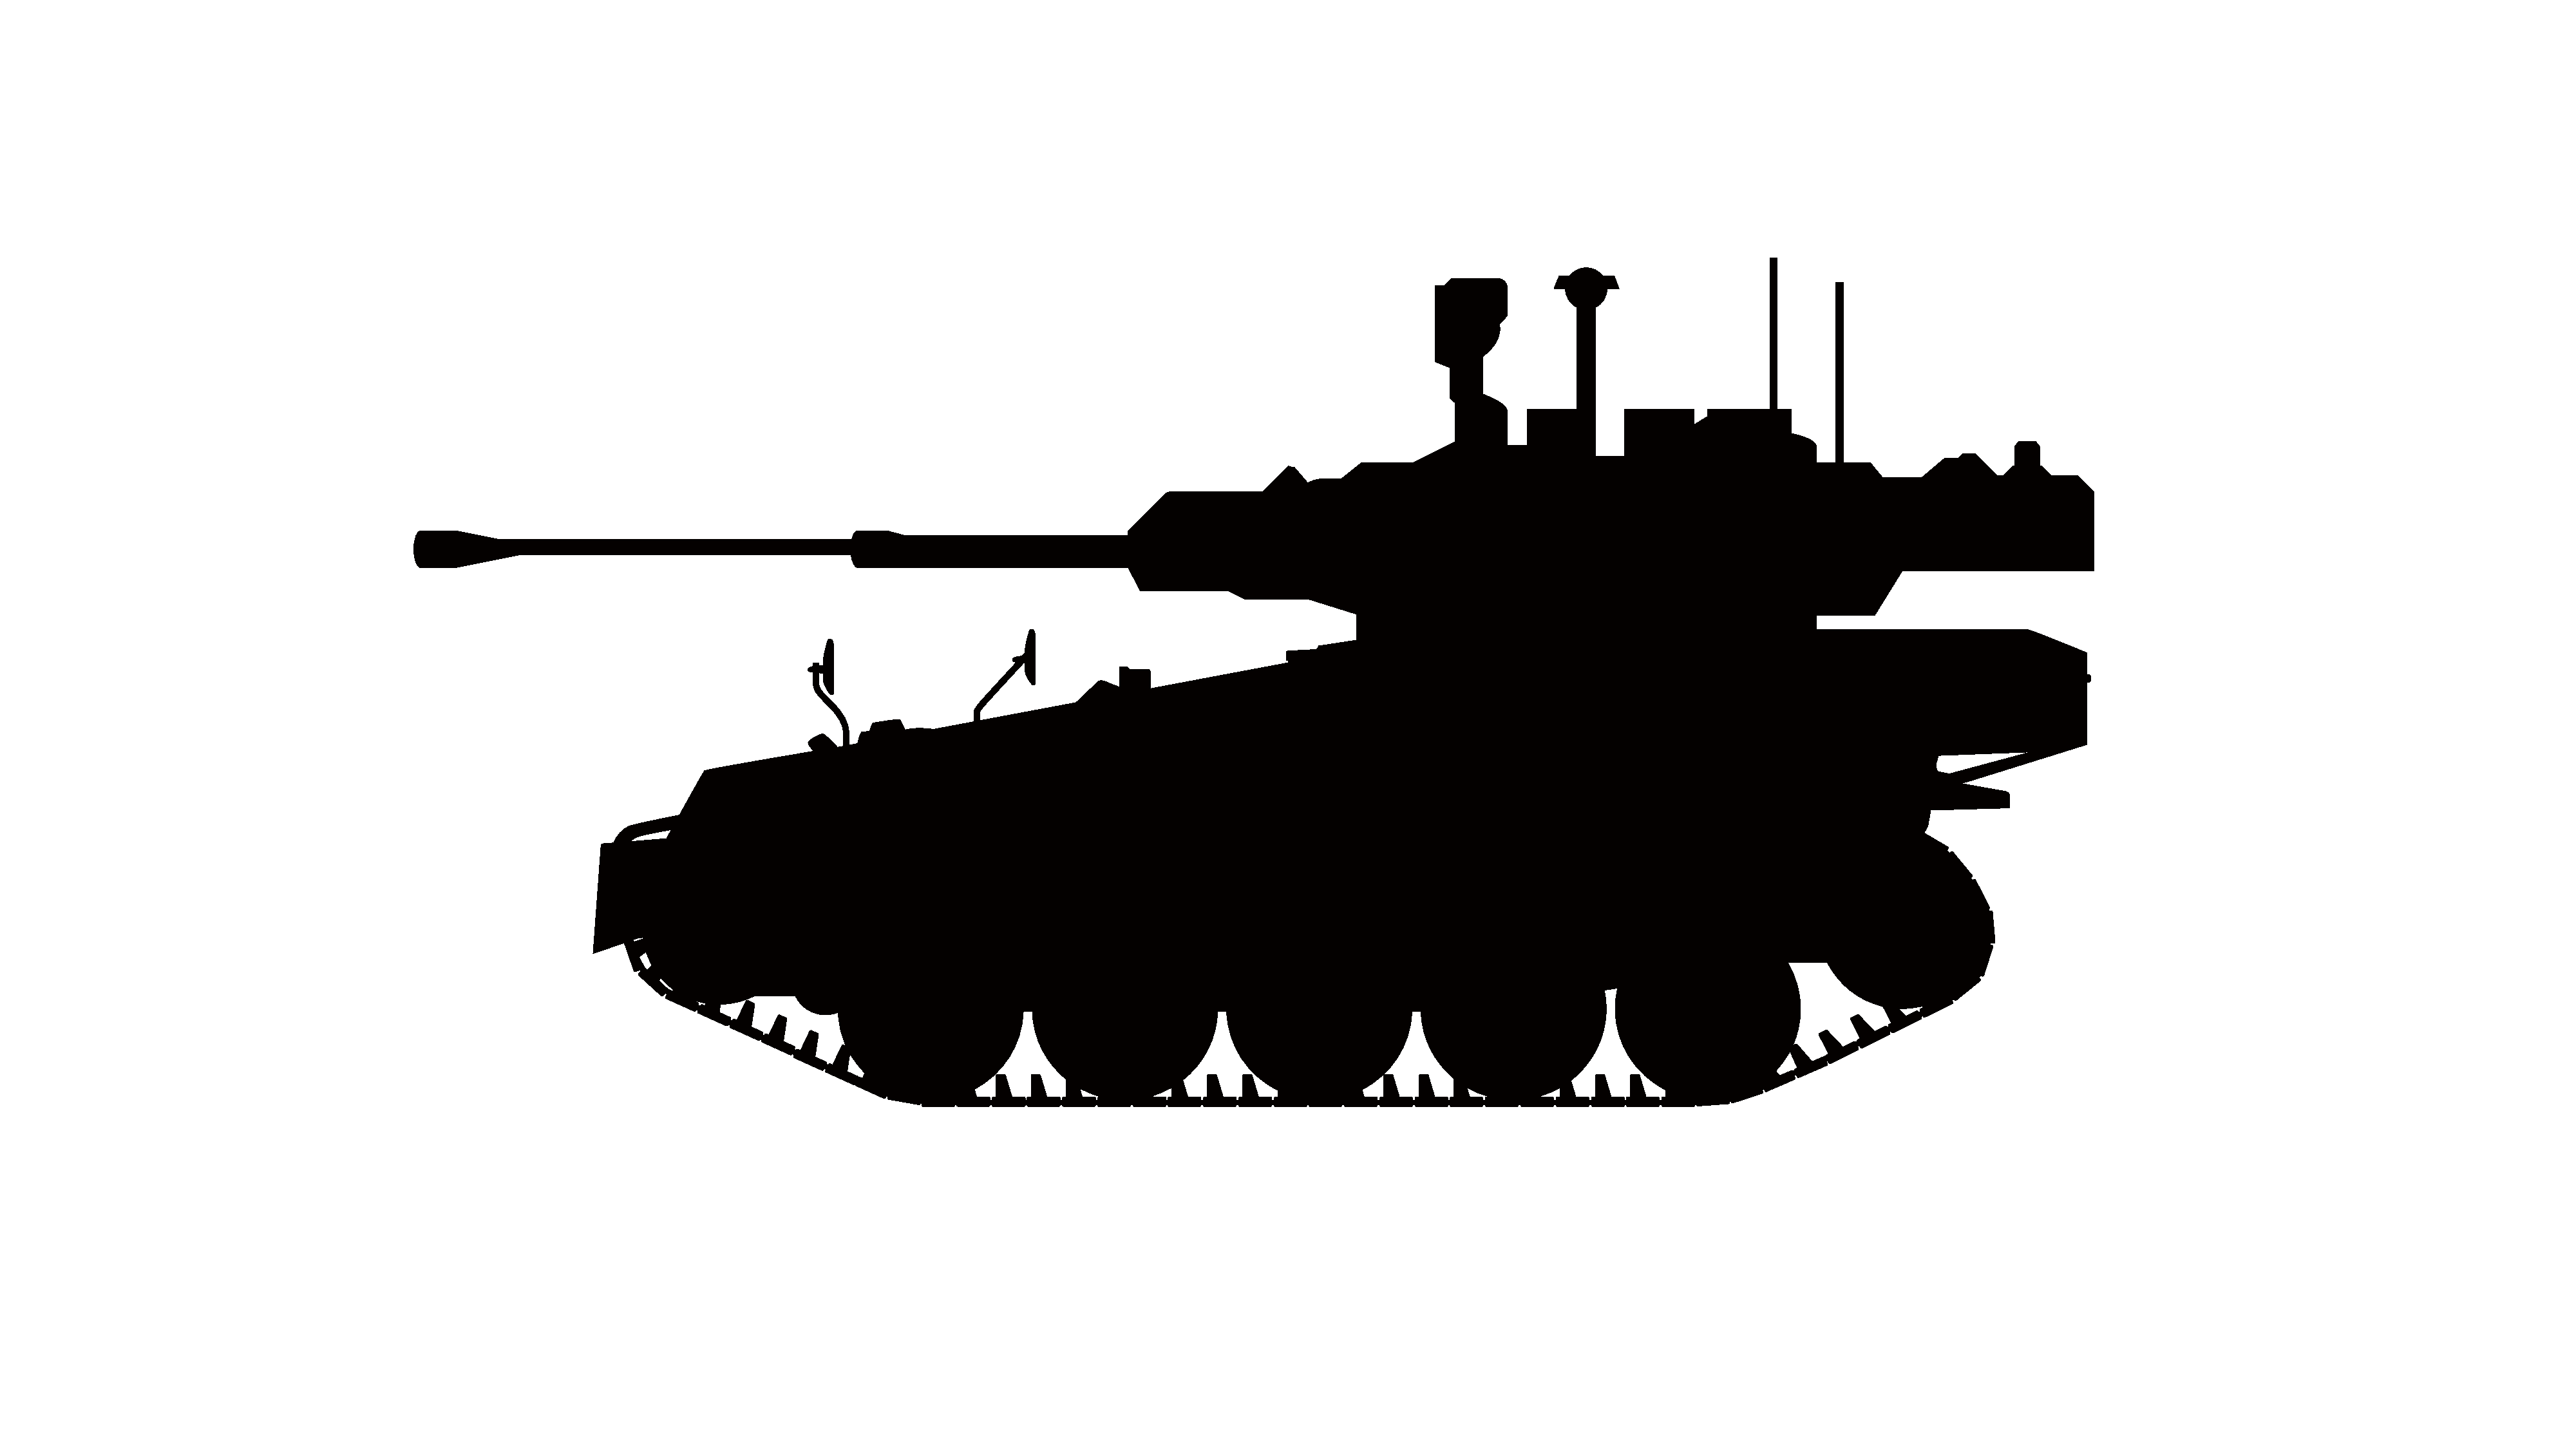
\includegraphics[width=0.7\textwidth]{platforms/sabre.pdf}
  \caption*{Sabre}
\end{figure}

\begin{figure}[h]
  \centering
  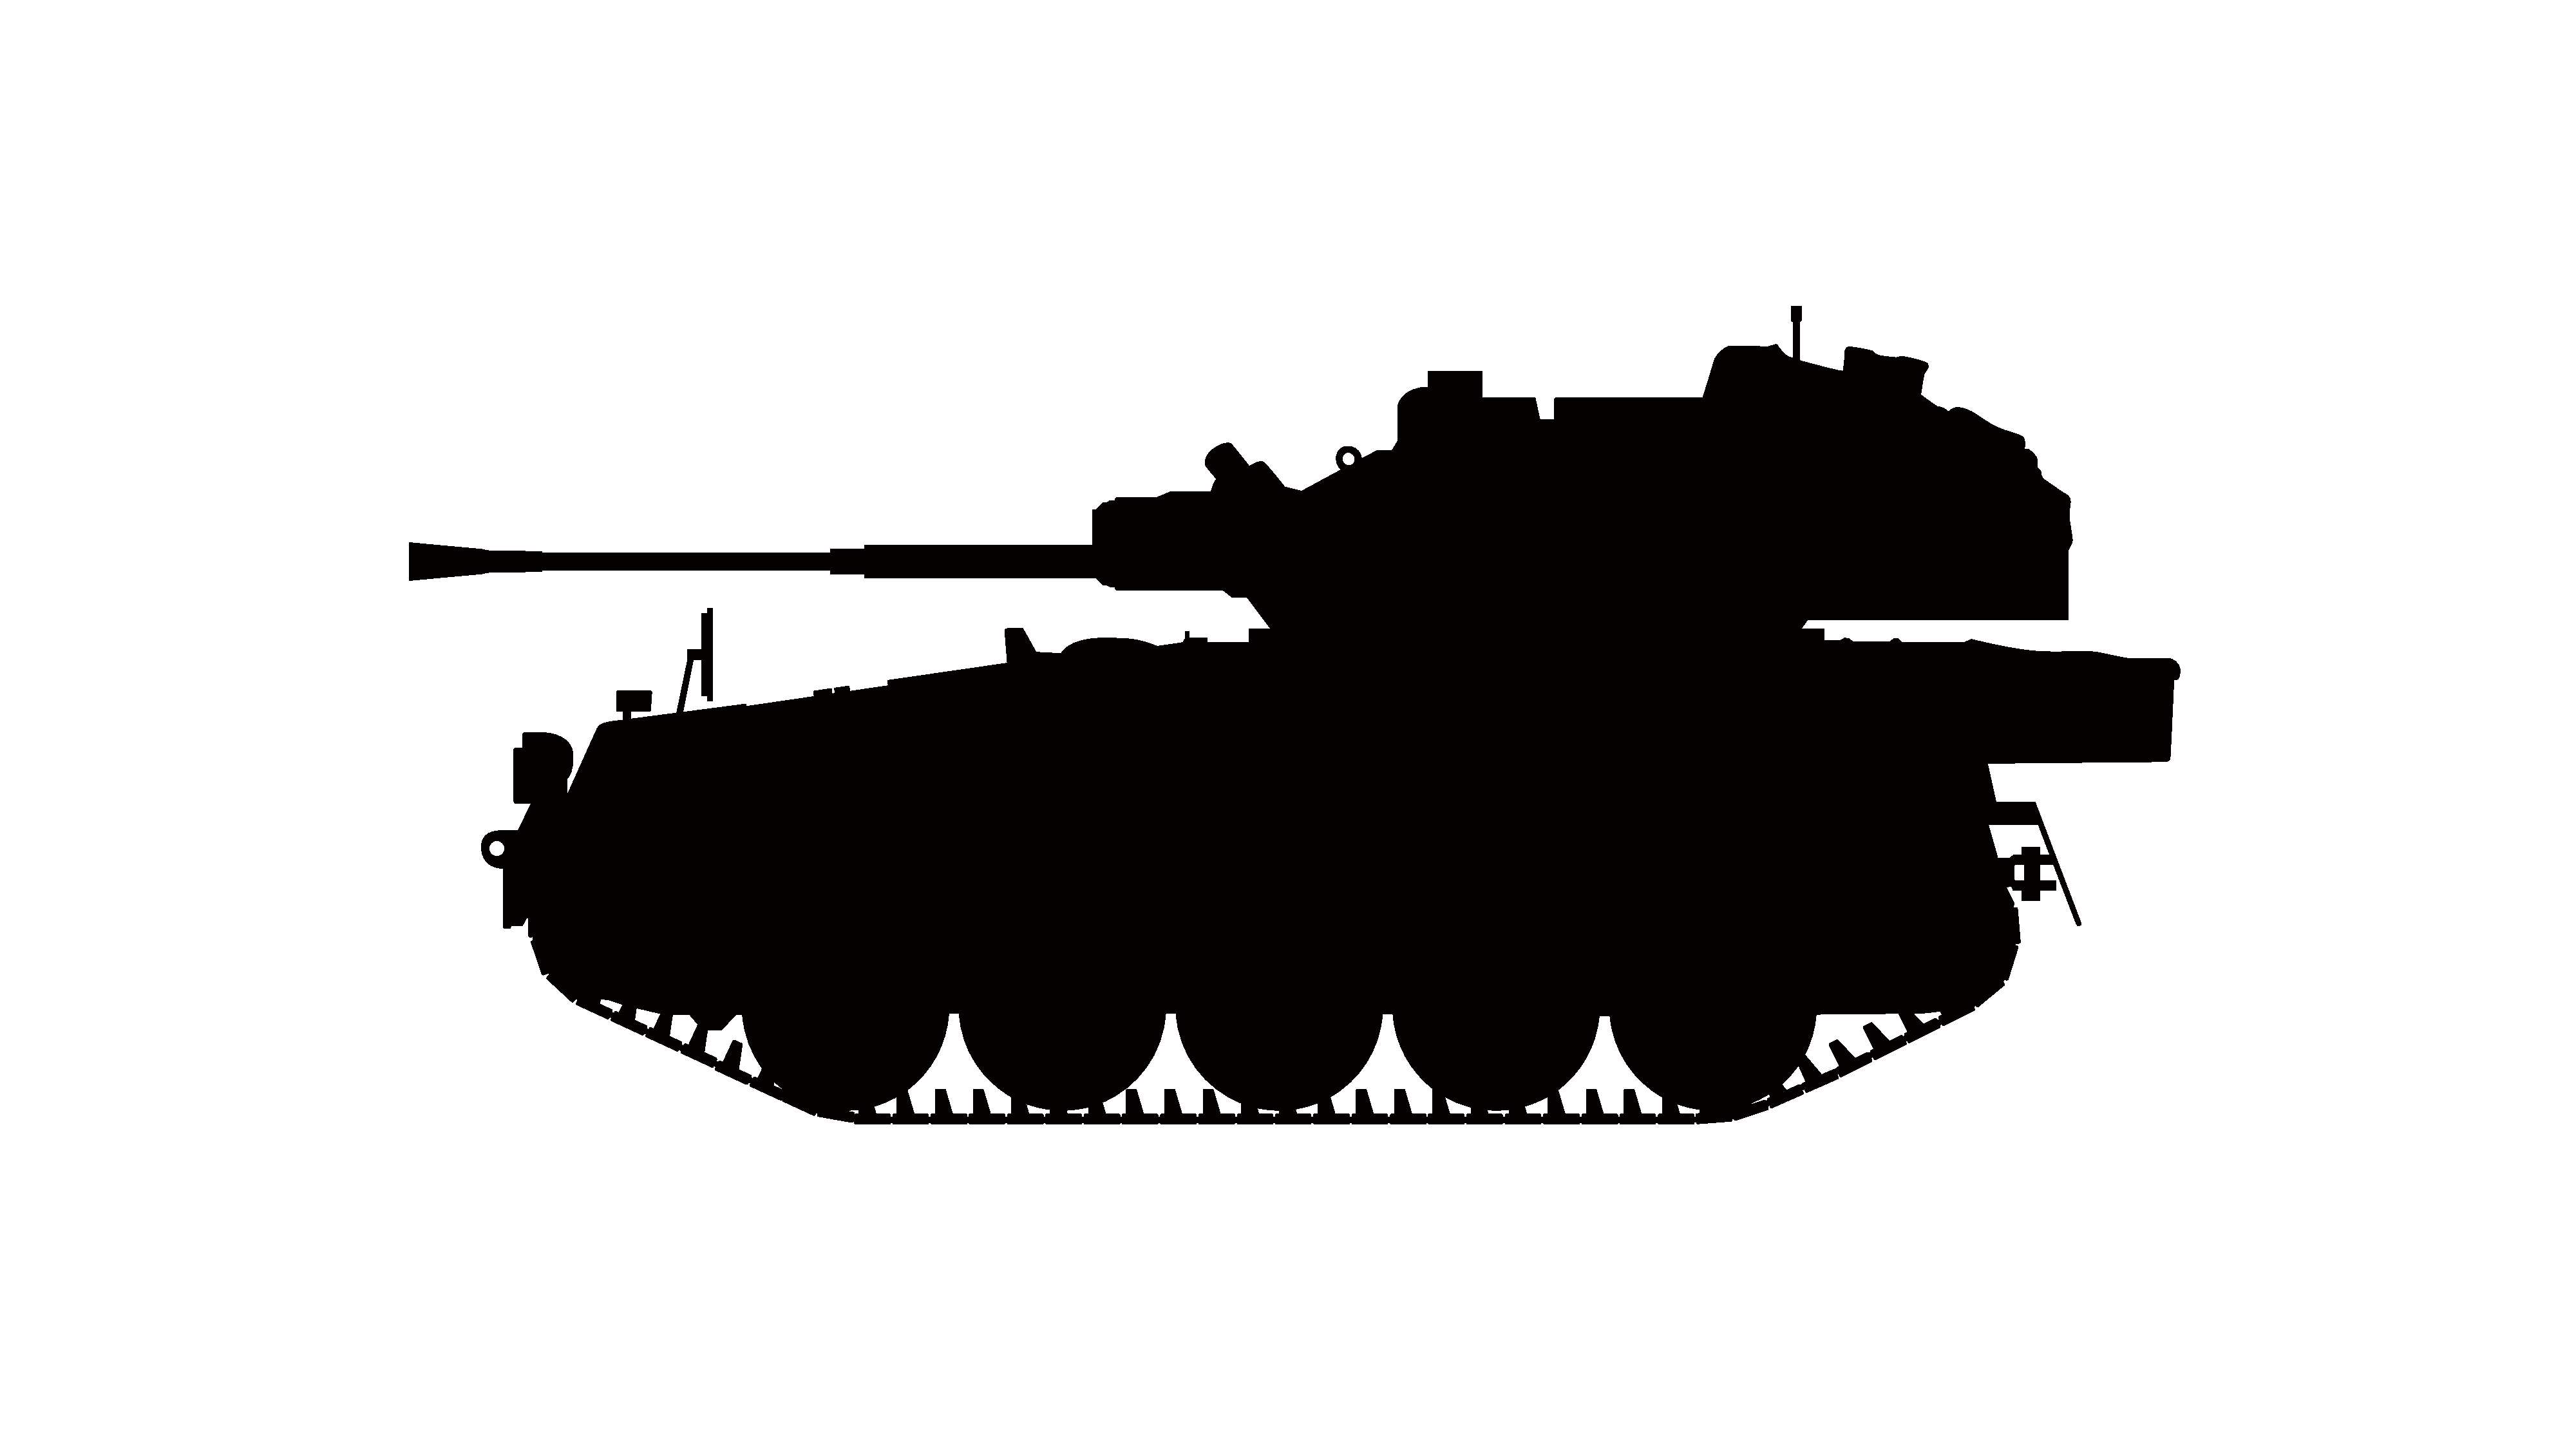
\includegraphics[width=0.7\textwidth]{platforms/scimitar.pdf}
  \caption*{Scimitar}
\end{figure}

\begin{figure}[h]
  \centering
  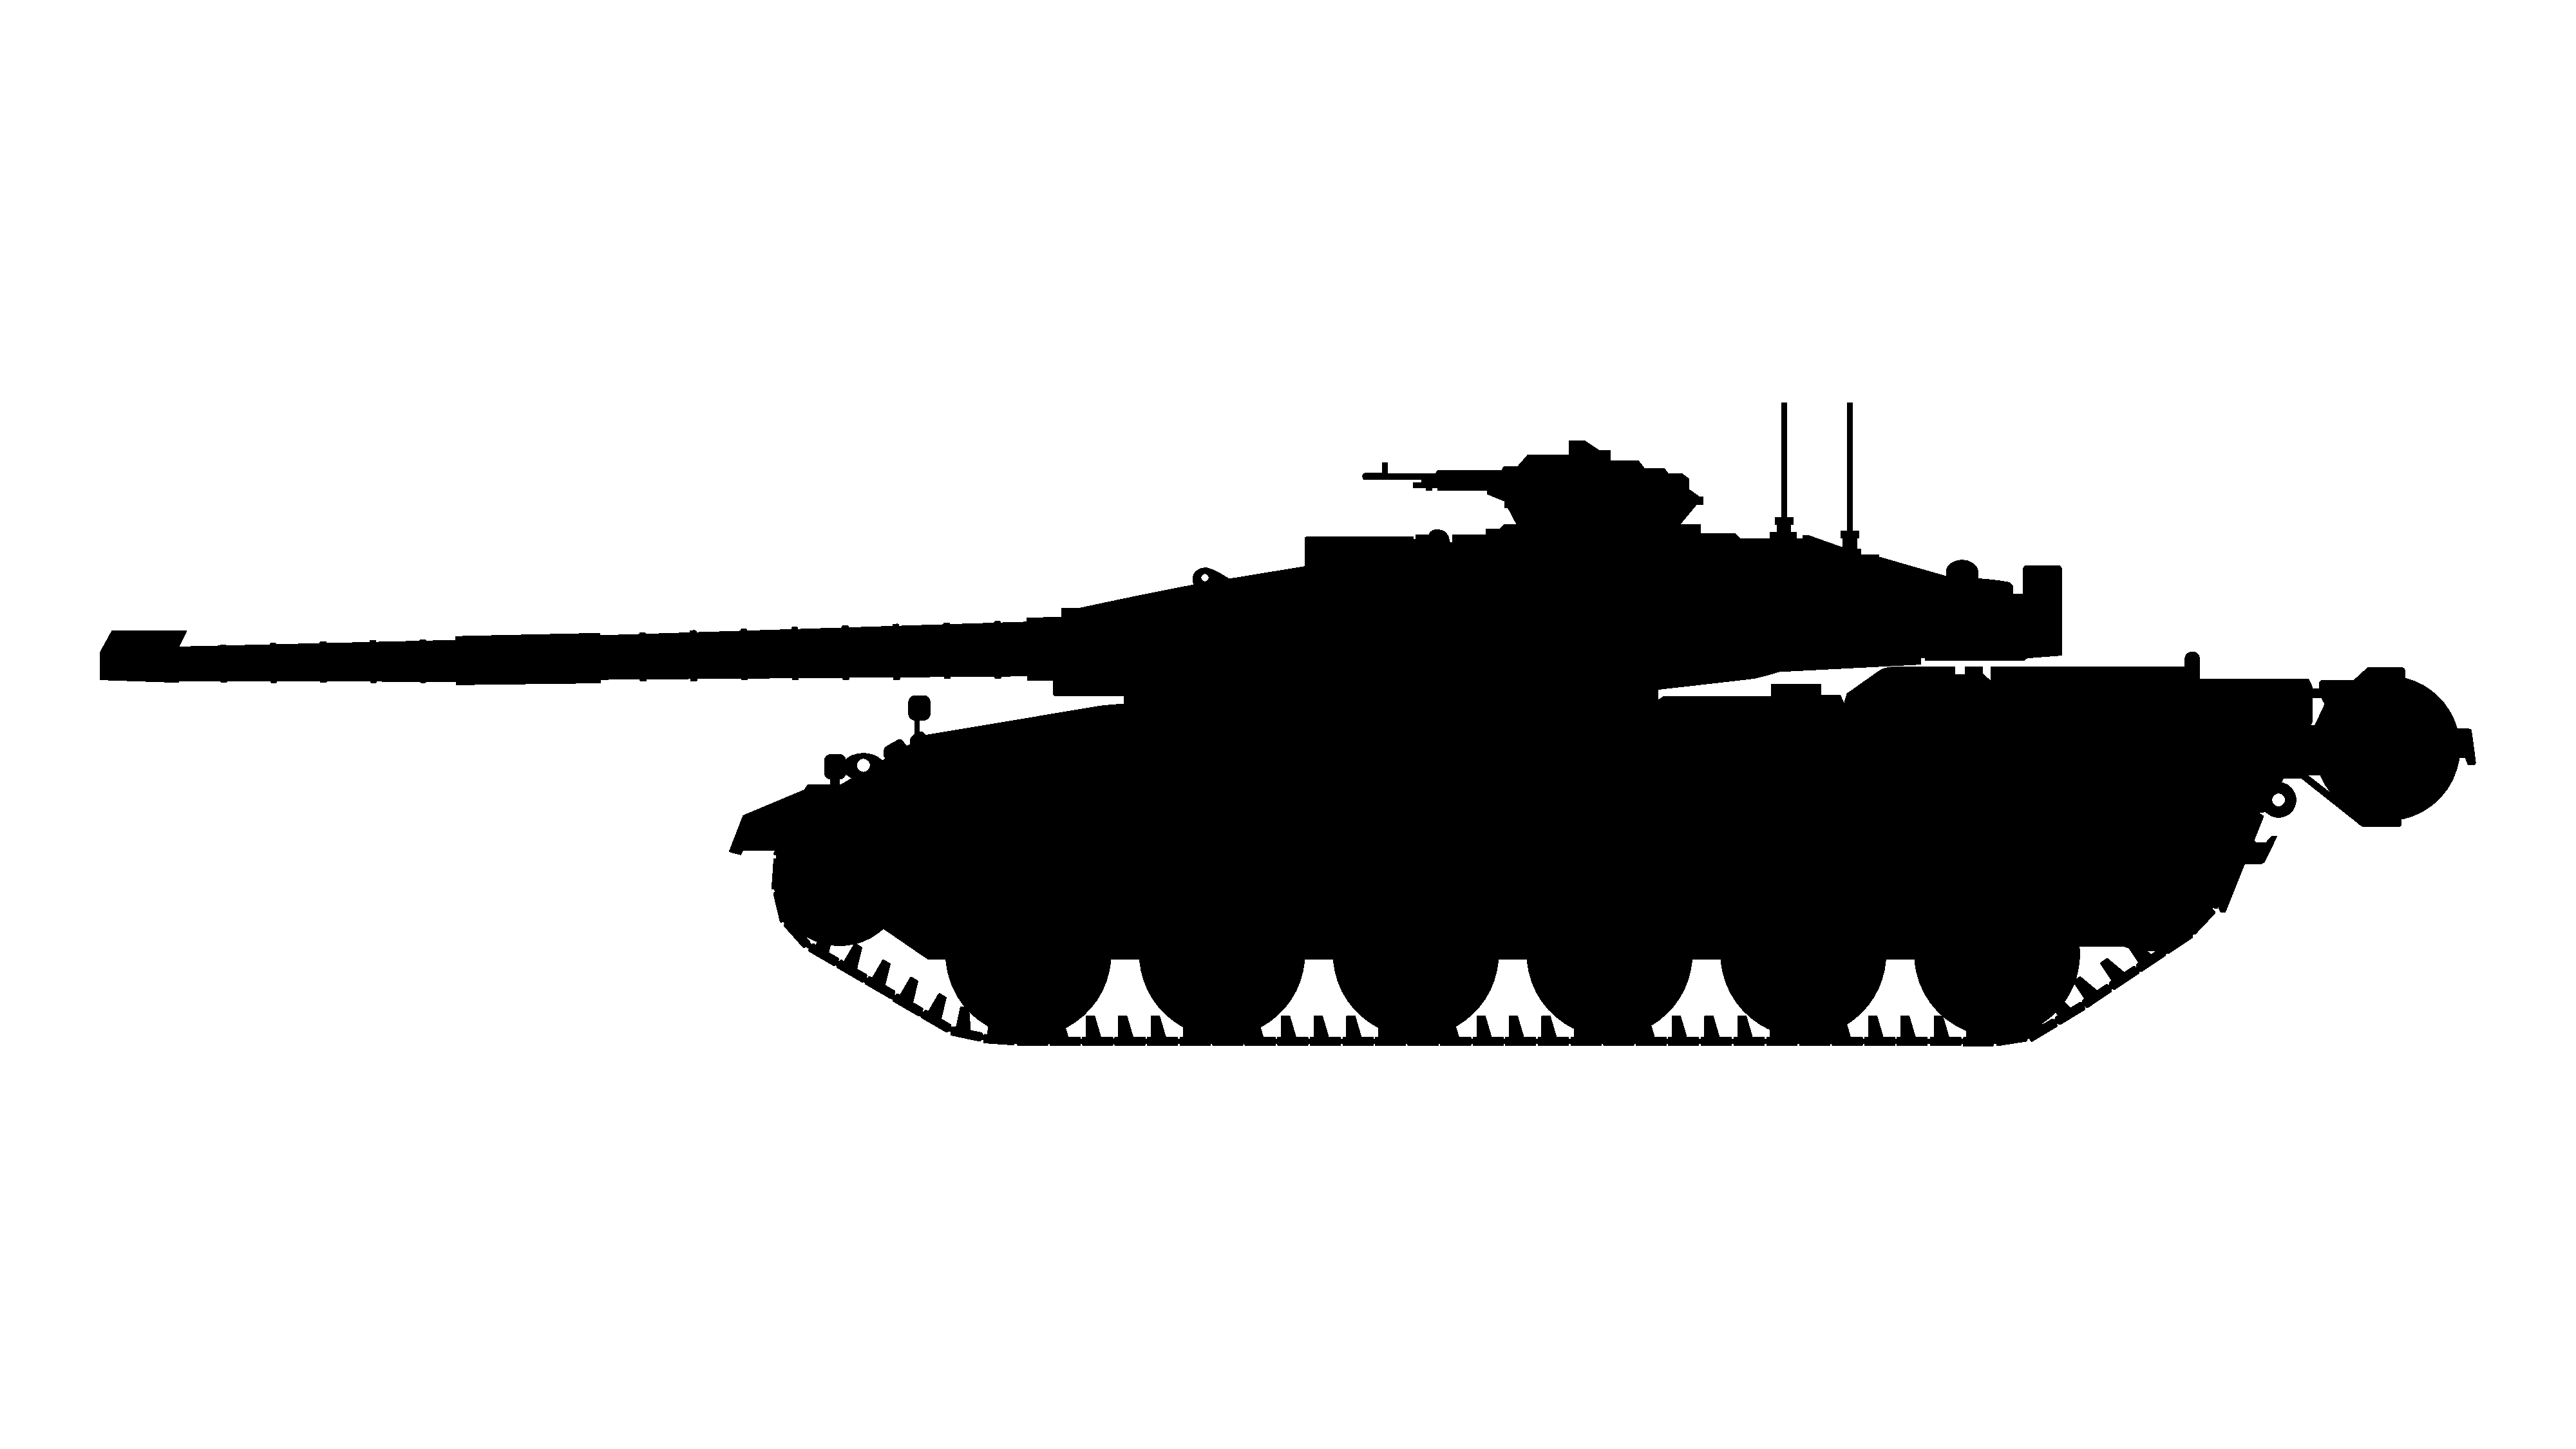
\includegraphics[width=0.7\textwidth]{platforms/challenger.pdf}
  \caption*{Challenger 2}
\end{figure}

\begin{figure}[h]
  \centering
  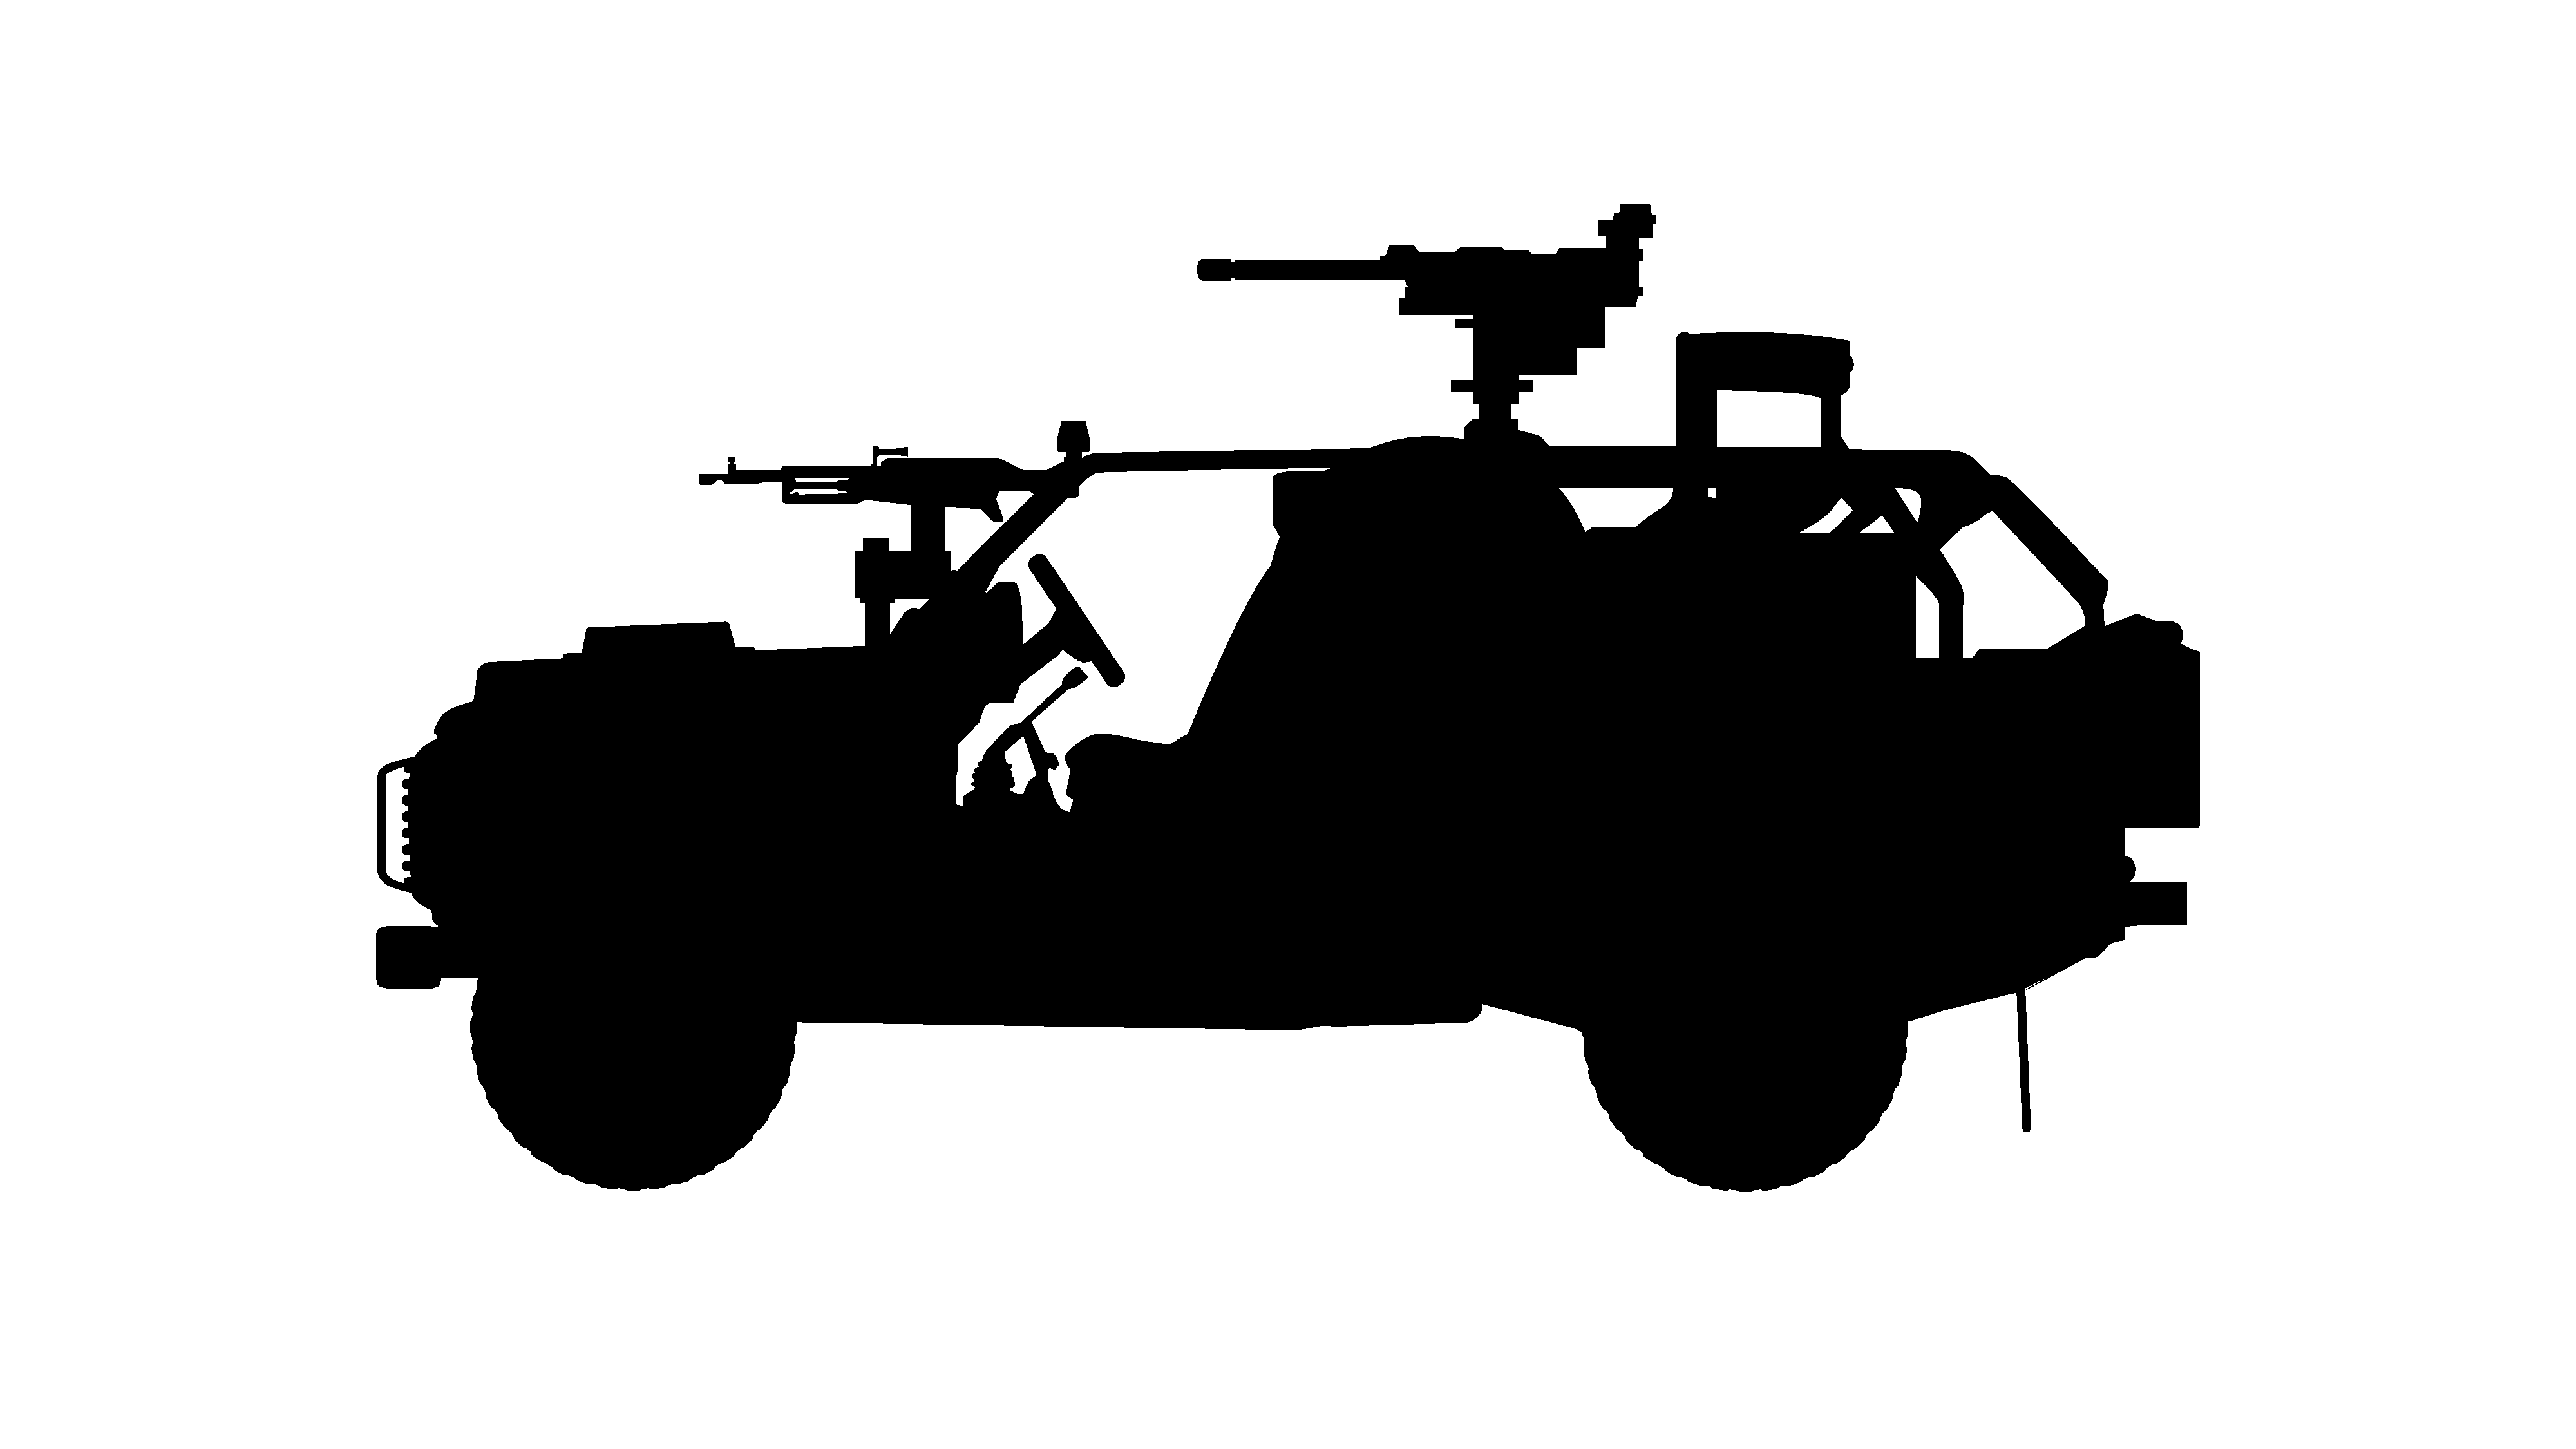
\includegraphics[width=0.7\textwidth]{platforms/wmik.pdf}
  \caption*{Land Rover Wolf RWMIK}
\end{figure}

\begin{figure}[h]
  \centering
  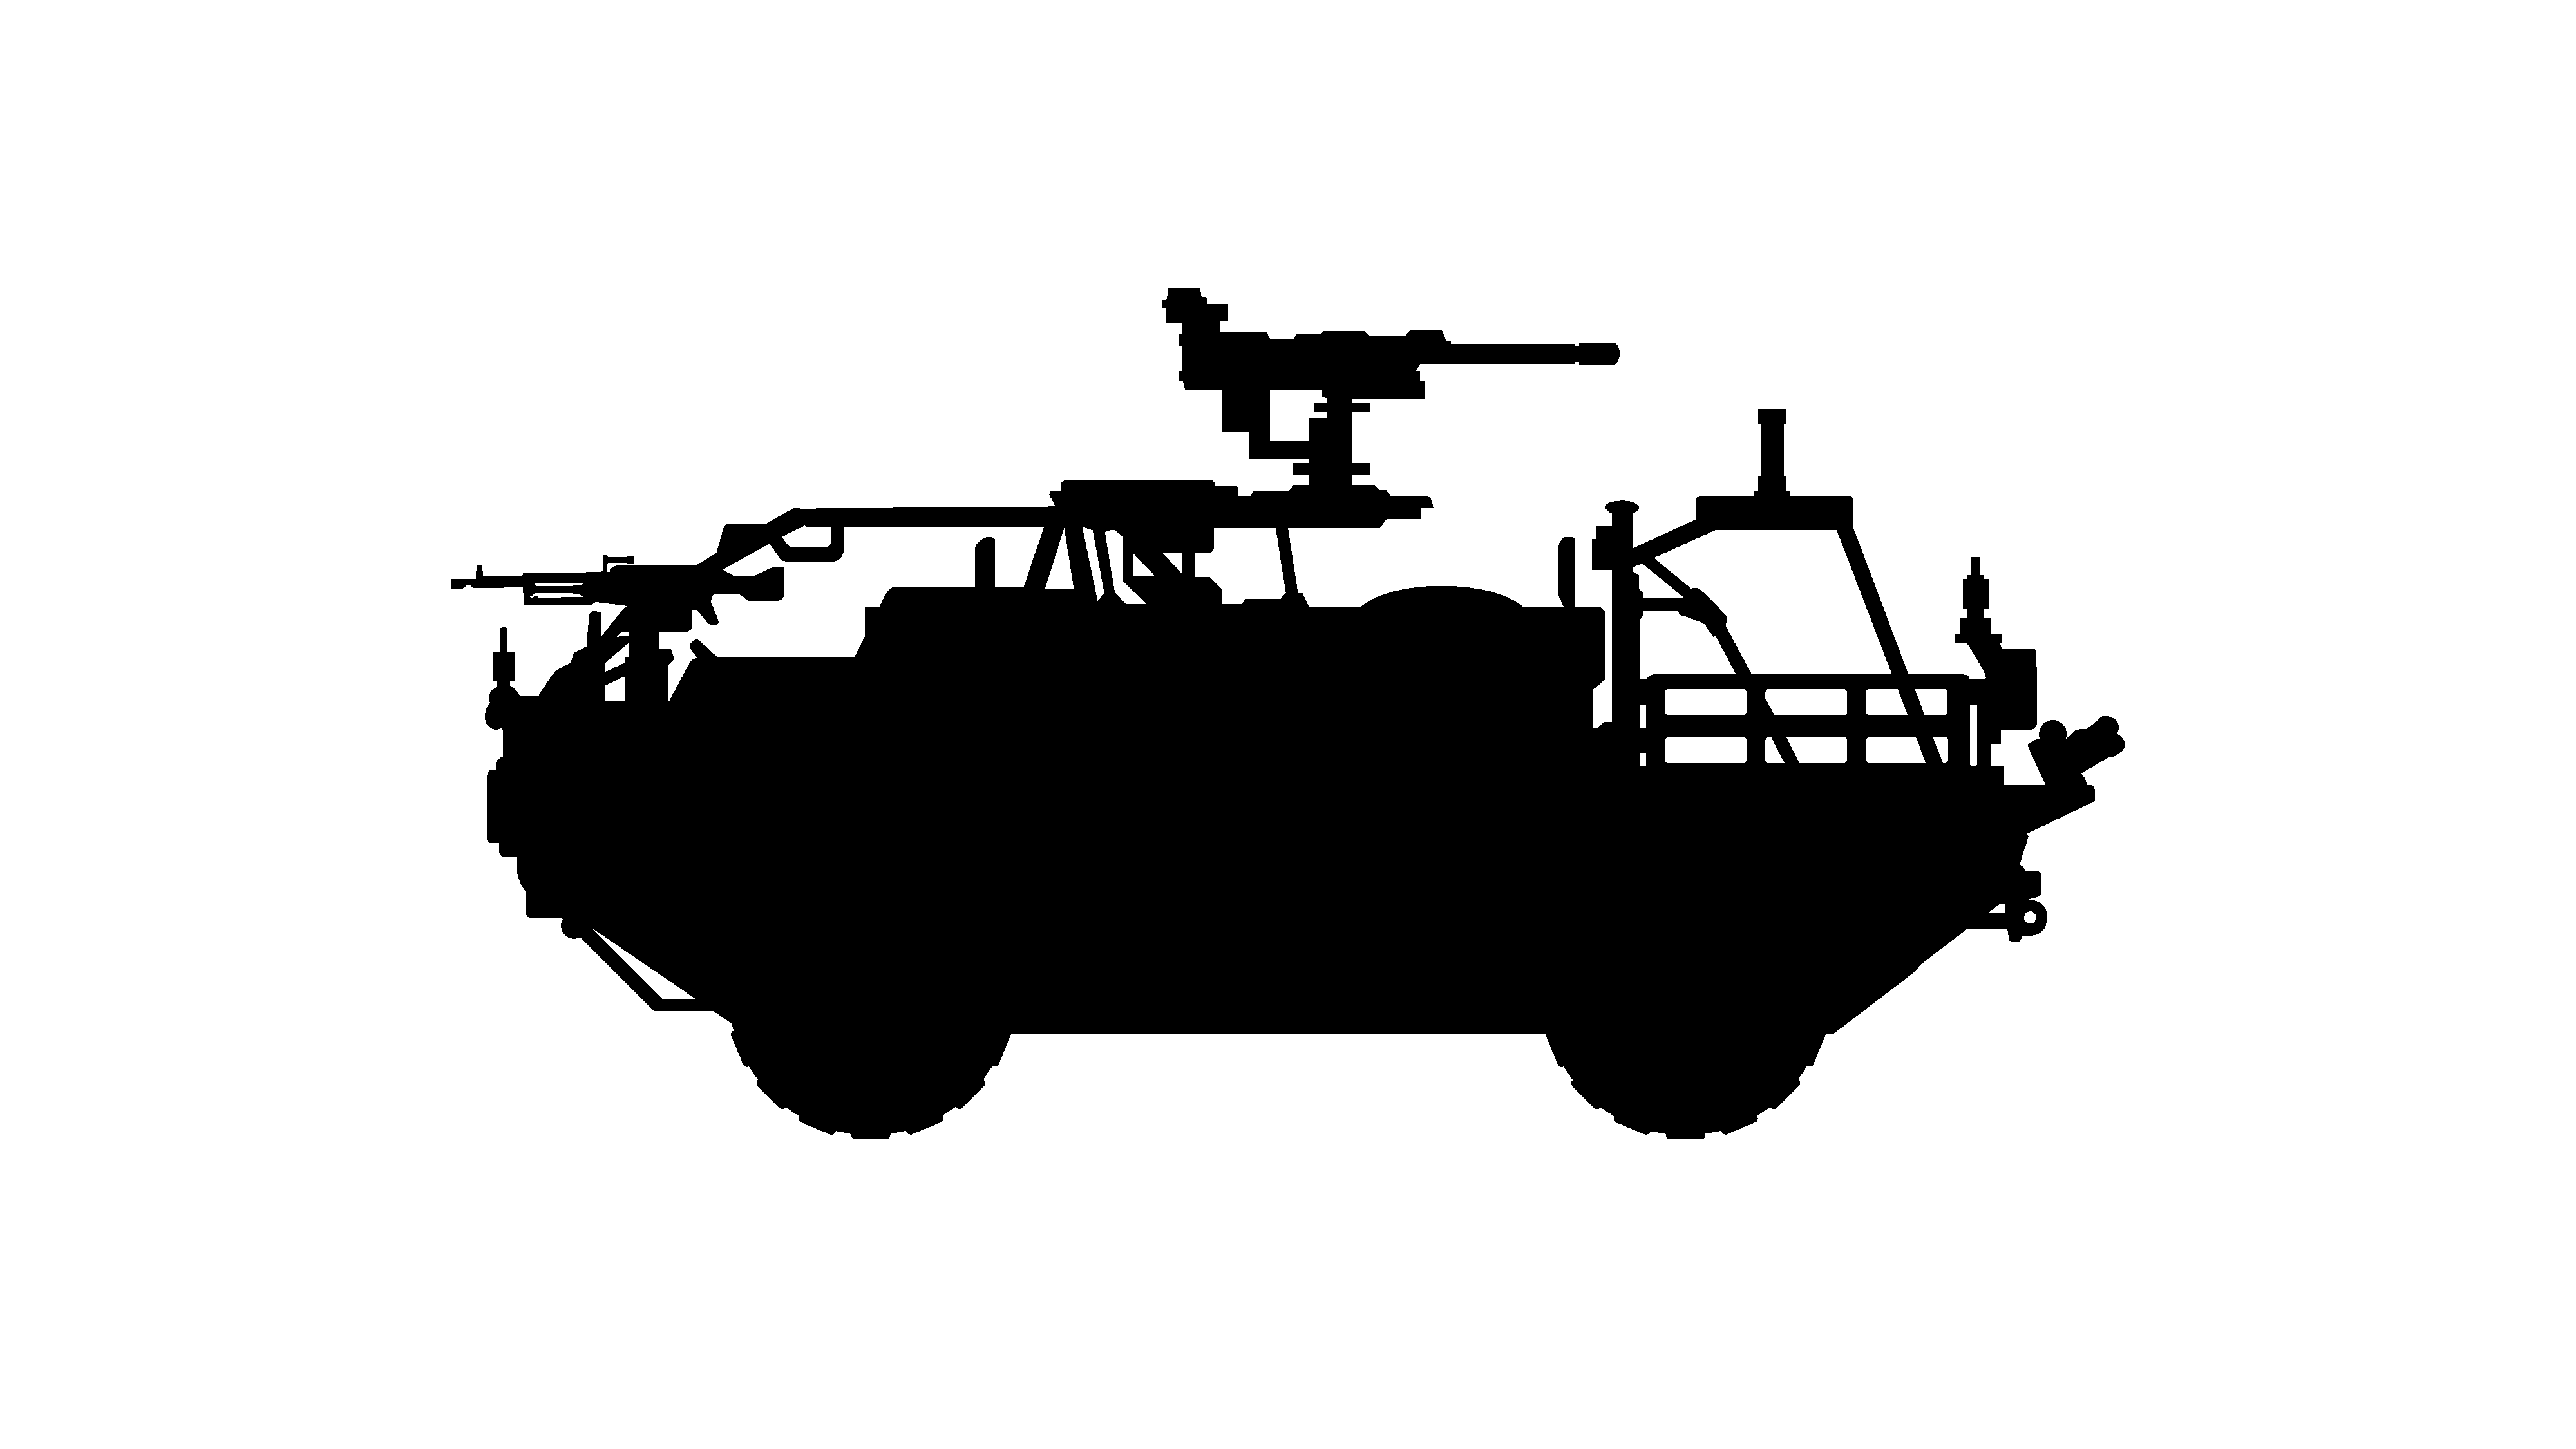
\includegraphics[width=0.7\textwidth]{platforms/jackal.pdf}
  \caption*{Supacat Jackal MWMIK}
\end{figure}

\chapter{Regimental Calls and March}

\begin{figure}[h]
  \centering
  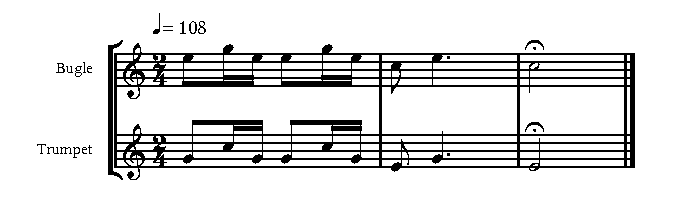
\includegraphics[width=\textwidth]{gazette/cheshire-yeomanry-call.pdf}
  \caption*{Regimental call of the Cheshire Yeomanry~\cite[p11]{trumpet-and-bugle-calls}}
\end{figure}

\vspace{10mm}

\begin{figure}[h]
  \centering
  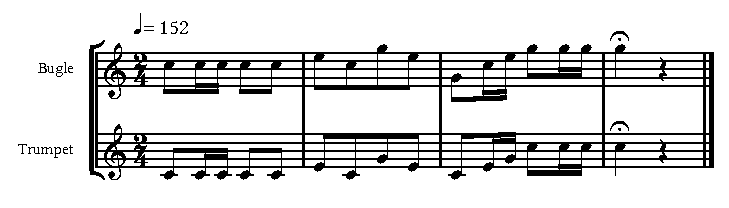
\includegraphics[width=\textwidth]{gazette/5ridg-call.pdf}
  \caption*{Regimental call of the 5\nth Royal Inniskilling Dragoon Guards~\cite[p3]{trumpet-and-bugle-calls}}
\end{figure}

\vfill

The Cheshire Yeomanry typically used the calls of the 5\nth Royal Inniskilling Dragoon Guards~\cite[p11]{trumpet-and-bugle-calls}, but also had their own calls.

\vfill

\pagebreak

\vspace*{10mm}

\poemtitle{D'ye ken John Peel}

\vfill

\begin{verse}[60mm]
\footnotesize
D'ye ken John Peel with his coat so gray? \\
D'ye ken John Peel at the break of the day? \\
D'ye ken John Peel when he's far, far away, \\
With his hounds and his horn in the morning?

\vin  'Twas the sound of his horn call'd me from my bed, \\
\vin  And the cry of his hounds has me oft-times led; \\
\vin  For Peel's view halloa would 'waken the dead, \\
\vin  Or a fox from his lair in the morning.

D'ye ken that bitch whose tongue is death? \\
D'ye ken her sons of peerless faith? \\
D'ye ken that a fox with his last breath \\
Curs'd them all as he died in the morning?

\vin  'Twas the sound of his horn call'd me from my bed...

Yes, I ken John Peel and auld Ruby, too, \\
Ranter and Royal and Bellman as true; \\
From the drag to the chase, from the chase to the view, \\
From the view to the death in the morning.

\vin  'Twas the sound of his horn call'd me from my bed...

And I've follow'd John Peel both often and far, \\
O'er the rasper-fence and the gate and the bar, \\
From Low Denton-holme up to the Scratchmere Scar, \\
When we vied for the brush in the morning.

\vin  'Twas the sound of his horn call'd me from my bed...

Then, here's to John Peel with my heart and soul, \\
Come fill--fill to him another strong bowl: \\
And we'll follow John Peel thro' fair and thro' foul \\
While we're wak'd by his horn in the morning.

\vin  'Twas the sound of his horn call'd me from my bed...
\end{verse}

\vfill

\begin{figure}[h]
  \centering
  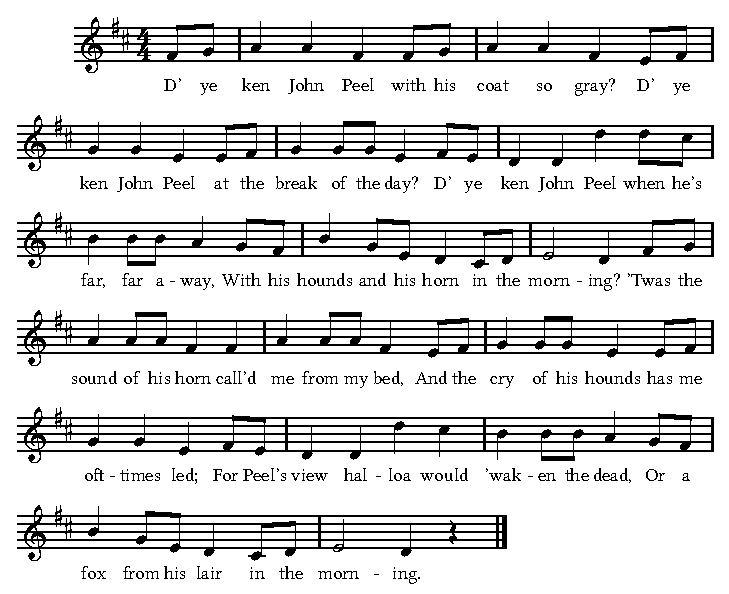
\includegraphics[width=\textwidth]{gazette/john-peel.pdf}
\end{figure}

\endgroup
